\documentclass{article}

% Formato base: el de la Tarea 1 (article 10 pt, carta, Latin Modern).
% Compilar con XeLaTeX o Tectonic:  tectonic Tarea_2_ONL.tex
\usepackage[spanish,es-tabla,es-nodecimaldot]{babel}
\usepackage{fontspec}
\usepackage{amsmath,amssymb,mathtools}
\usepackage{graphicx}
\usepackage{booktabs}
\usepackage{siunitx}
\usepackage{xcolor}
\usepackage{float}
\usepackage{tikz}
\usetikzlibrary{babel,angles,quotes,arrows.meta,calc}
\usepackage{listings}
\usepackage[margin=2.4cm]{geometry}
\usepackage{hyperref}

\sisetup{output-decimal-marker={.}, per-mode=symbol, range-phrase={--}}
\hypersetup{colorlinks=true, linkcolor=black, citecolor=black, urlcolor=black}
\graphicspath{{figuras/}}

\lstset{basicstyle=\ttfamily\scriptsize, breaklines=true, columns=fullflexible,
  keepspaces=true, frame=single, numbers=left, numberstyle=\tiny, numbersep=5pt,
  commentstyle=\color{green!45!black}, keywordstyle=\color{blue!70!black},
  language=Matlab, inputencoding=utf8, extendedchars=true,
  literate={á}{{\'a}}1 {é}{{\'e}}1 {í}{{\'i}}1 {ó}{{\'o}}1 {ú}{{\'u}}1 {ñ}{{\~n}}1
           {Á}{{\'A}}1 {É}{{\'E}}1 {Í}{{\'I}}1 {Ó}{{\'O}}1 {Ú}{{\'U}}1 {Ñ}{{\~N}}1 {ü}{{\"u}}1}

% Notación de Saleh: campos reales en caligráfica, amplitudes complejas en negrita.
\newcommand{\Ec}{\boldsymbol{\mathcal{E}}}
\newcommand{\Pc}{\boldsymbol{\mathcal{P}}}
\newcommand{\dd}{\,\mathrm{d}}
\newcommand{\xh}{\hat{\mathbf{x}}}
\newcommand{\yh}{\hat{\mathbf{y}}}
\newcommand{\zh}{\hat{\mathbf{z}}}
\newcommand{\kv}{\mathbf{k}}
\newcommand{\Sv}{\mathbf{S}}
\newcommand{\Ev}{\mathbf{E}}
\newcommand{\Dv}{\mathbf{D}}
\newcommand{\Jv}{\mathbf{J}}
\newcommand{\Tm}{\mathbf{T}}
\newcommand{\Rm}{\mathbf{R}}
\newcommand{\Pm}{\mathbf{P}}
\newcommand{\Dnu}{D_\nu}
\newcommand{\Dlam}{D_\lambda}
\newcommand{\um}{\si{\micro\metre}}
\newcommand{\pskmnm}{\si{\pico\second\per\kilo\metre\per\nano\metre}}

\title{Tarea 2: dispersión, propagación de pulsos y óptica de polarización}
\author{Juan E. Rodriguez Ochoa\\
Profesor: Rodrigo Acuña Herrera\\
Óptica No Lineal, Escuela de Física\\
Universidad Nacional de Colombia, Sede Medellín}
\date{Noviembre 2026}

\begin{document}
\maketitle

\noindent\textbf{Convenciones.} Se usan unidades SI y la notación de Saleh y Teich,
\emph{Fundamentals of Photonics}, 2.ª ed. (Wiley, 2007), que es la edición a la que remiten
los números de ejercicio del enunciado. Los campos reales se escriben $\Ec(\mathbf r,t)$, las
amplitudes complejas $\Ev(\mathbf r)$, la dependencia temporal es $e^{j\omega t}$ y
$j=\sqrt{-1}$. Con esta convención una onda que viaja en $+z$ es $e^{-jkz}$, la
transformada de Fourier es $F[f](\nu)=\int f(t)\,e^{-j2\pi\nu t}\dd t$ (ec.~A.1-2) y la parte
imaginaria de la susceptibilidad de un medio absorbente es \emph{negativa}
($\chi''<0\Rightarrow\alpha>0$, §5.5A). Las constantes usadas son $c_0=\SI{2.99792458e8}{m/s}$ y
$k_0=\omega/c_0=2\pi/\lambda_0$. Las ecuaciones citadas como (5.5-27), (6.2-12), etc.\ son las del
libro.

\medskip
\noindent\textbf{Nota sobre el punto 3.} El enunciado lo etiqueta ``[Problema 5.6-3]''. En la
2.ª edición el problema 5.6-3 (p.~196) es ``Group Velocity in a Metal''; el enunciado del punto 3
parece seguir la numeración de la 1.ª edición, que la 2.ª edición no conserva. Como el
enunciado es autocontenido, se resuelve tal como está escrito. Además, la fibra ``hecha de
silicio'' es de \emph{sílice} fundida (SiO$_2$), que es el material de la Fig.~5.6-5; el silicio
cristalino es opaco por debajo de \SI{1.1}{\um} y no se usa en fibras.

%=====================================================================
\section{Punto 1: Ejercicio 5.5-1, medio absorbente diluido}
%=====================================================================

\emph{Un medio no absorbente de índice de refracción $n_0$ aloja una suspensión diluida de
impurezas caracterizadas por una susceptibilidad $\chi=\chi'+j\chi''$, con $\chi'\ll1$ y
$\chi''\ll1$. Determine la susceptibilidad total del medio y demuestre que el índice de
refracción y el coeficiente de absorción están dados aproximadamente por
$n\approx n_0+\chi'/2n_0$ (5.5-9) y $\alpha\approx-k_0\chi''/n_0$ (5.5-10).} (Saleh y Teich,
p.~172--173.)

\subsection*{Susceptibilidad total}

El medio anfitrión es un dieléctrico lineal, homogéneo, isótropo y sin pérdidas, de modo que su
polarización es $\Pc_{\rm h}=\epsilon_0\chi_{\rm h}\Ec$ con $\chi_{\rm h}$ real. Su índice es
$n_0=\sqrt{1+\chi_{\rm h}}$ (ec.~5.2-13), luego
\[
\chi_{\rm h}=n_0^2-1 .
\]
Las impurezas aportan una polarización adicional $\Pc_{\rm i}=\epsilon_0\chi\Ec$. Que la
suspensión sea \emph{diluida} significa dos cosas: (i) el campo que actúa sobre cada impureza es
el campo macroscópico $\Ec$ (no hay corrección de campo local apreciable), y (ii) la respuesta
de las impurezas no modifica la del anfitrión. En un medio lineal las polarizaciones se
superponen, así que
\[
\Pc=\Pc_{\rm h}+\Pc_{\rm i}=\epsilon_0\left(\chi_{\rm h}+\chi\right)\Ec
\quad\Longrightarrow\quad
\boxed{\;\chi_{\rm tot}=\chi_{\rm h}+\chi=\left(n_0^2-1\right)+\chi'+j\chi''\;}
\]
Es decir, la susceptibilidad total tiene parte real $n_0^2-1+\chi'$ y parte imaginaria $\chi''$:
toda la absorción proviene de las impurezas.

\subsection*{Índice y coeficiente de absorción}

La relación general entre $(n,\alpha)$ y la susceptibilidad compleja es la ec.~(5.5-5),
\[
n-j\frac{\alpha}{2k_0}=\sqrt{1+\chi_{\rm tot}}
=\sqrt{n_0^2+\chi'+j\chi''}
= n_0\sqrt{1+\frac{\chi'+j\chi''}{n_0^2}} .
\]
Como $|\chi'+j\chi''|\ll1\le n_0^2$, el cociente $x=(\chi'+j\chi'')/n_0^2$ es pequeño y se puede
usar la expansión binomial $\sqrt{1+x}=1+\tfrac12x-\tfrac18x^2+\cdots$ truncada en el primer
orden (el error es de orden $|x|^2/8$):
\[
n-j\frac{\alpha}{2k_0}\approx n_0\left(1+\frac{\chi'+j\chi''}{2n_0^2}\right)
= n_0+\frac{\chi'}{2n_0}+j\frac{\chi''}{2n_0}.
\]
Igualando partes reales e imaginarias:
\[
\boxed{\,n\approx n_0+\frac{\chi'}{2n_0}\,}\qquad(5.5\text{-}9),
\qquad\qquad
-\frac{\alpha}{2k_0}=\frac{\chi''}{2n_0}\;\Longrightarrow\;
\boxed{\,\alpha\approx-\frac{k_0\chi''}{n_0}\,}\qquad(5.5\text{-}10).
\]

\subsection*{Comentarios}

\begin{itemize}
\item Para $n_0=1$ (impurezas en el vacío) se recuperan las fórmulas del medio débilmente
absorbente, (5.5-7) y (5.5-8): $n\approx\sqrt{1+\chi'}\approx1+\chi'/2$ y
$\alpha\approx-k_0\chi''$ (la (5.5-8) es $\alpha\approx-k_0\chi''/n$, con $n\approx1$ en este caso).
\item El signo es consistente con la convención del libro: en un medio absorbente $\chi''<0$,
luego $\alpha>0$ y la onda $e^{-\alpha z/2}e^{-j\beta z}$ se atenúa. En un medio con ganancia
$\chi''>0$ y $\alpha<0$.
\item Escribiendo $k_0=2\pi\nu/c_0$ se obtiene exactamente la forma (5.5-26)--(5.5-27) que el
libro usa para el medio resonante diluido,
$\alpha(\nu)\approx-(2\pi\nu/n_0c_0)\,\chi''(\nu)$ y $n(\nu)\approx n_0+\chi'(\nu)/2n_0$.
Esta es la base del punto 2.
\item La presencia del anfitrión \emph{reduce} ambos efectos en un factor $n_0$, por razones
distintas. En el índice, $\chi'$ cambia $n^2$ y $\Delta n=\Delta(n^2)/2n_0=\chi'/2n_0$. En la
absorción, el campo de una onda de intensidad dada es menor en un medio de índice alto,
$|E|^2=2\eta I=2\eta_0I/n_0$, y la potencia absorbida por unidad de volumen, proporcional a
$|\chi''||E|^2$, disminuye en ese mismo factor.
\end{itemize}

%=====================================================================
\section{Punto 2: velocidad de grupo de un medio resonante}
%=====================================================================

\emph{Determinar una expresión para la velocidad de grupo de un medio resonante con índice de
refracción dado por las ecuaciones (5.5-27), (5.5-23) y (5.5-24). Dibujar a mano alzada la
velocidad de grupo en función de la frecuencia e identificar regiones de dispersión normal y
anómala.}

\subsection*{Índice de refracción cerca de la resonancia}

Las ecuaciones de partida (Saleh y Teich, p.~178) son, cerca de la resonancia
($|\nu-\nu_0|\ll\nu_0$),
\begin{align}
\chi''(\nu)&\approx-\chi_0\frac{\nu_0\Delta\nu}{4}\,
\frac{1}{(\nu_0-\nu)^2+(\Delta\nu/2)^2}, \tag{5.5-23}\\
\chi'(\nu)&\approx2\,\frac{\nu-\nu_0}{\Delta\nu}\,\chi''(\nu), \tag{5.5-24}\\
n(\nu)&\approx n_0+\frac{\chi'(\nu)}{2n_0}, \tag{5.5-27}
\end{align}
donde $\nu_0$ es la frecuencia de resonancia, $\Delta\nu$ el ancho total a media altura de la
línea lorentziana, $\chi_0$ la susceptibilidad a baja frecuencia y $n_0$ el índice del anfitrión
(la última ecuación es el resultado del punto 1). Conviene definir la desintonía y la semianchura
\[
\delta\equiv\nu-\nu_0,\qquad a\equiv\frac{\Delta\nu}{2},\qquad Q\equiv\frac{\nu_0}{\Delta\nu}\gg1 .
\]
Sustituyendo (5.5-23) en (5.5-24):
\[
\chi'(\nu)=\frac{2\delta}{\Delta\nu}\left(-\chi_0\frac{\nu_0\Delta\nu}{4}\right)\frac{1}{\delta^2+a^2}
=-\frac{\chi_0\nu_0}{2}\,\frac{\delta}{\delta^2+a^2},
\]
y con (5.5-27)
\begin{equation}
n(\nu)=n_0-\frac{\chi_0\nu_0}{4n_0}\,\frac{\delta}{\delta^2+a^2}.
\label{eq:n_res}
\end{equation}
Esta es la curva dispersiva de la Fig.~5.5-7: $n=n_0$ en resonancia, máximo en $\delta=-a$ y
mínimo en $\delta=+a$ (los puntos donde $|\chi''|$ cae a la mitad de su valor máximo). En esta
aproximación $n\to n_0$ lejos de la línea; muy por debajo de $\nu_0$ el modelo completo da
$n\to n_0+\chi_0/2n_0$, el escalón que marca la figura.

\subsection*{Índice de grupo y velocidad de grupo}

La velocidad de grupo es $v=1/\beta'=\left(d\beta/d\omega\right)^{-1}$ (5.6-1) con
$\beta=\omega n(\omega)/c_0$. En términos de la frecuencia $\nu=\omega/2\pi$,
\[
\frac{1}{v}=\frac{d\beta}{d\omega}=\frac{1}{c_0}\frac{d}{d\nu}\left[\nu\,n(\nu)\right]
=\frac{1}{c_0}\left(n+\nu\frac{dn}{d\nu}\right)\equiv\frac{N}{c_0},
\qquad N=n+\nu\frac{dn}{d\nu}.
\]
Esta forma es equivalente a la (5.6-2), $N=n-\lambda_0\,dn/d\lambda_0$, porque
$\lambda_0=c_0/\nu$ implica $d\lambda_0=-(c_0/\nu^2)d\nu$ y por tanto
$-\lambda_0\,dn/d\lambda_0=\nu\,dn/d\nu$. Derivando \eqref{eq:n_res} respecto a $\nu$
($d\delta=d\nu$):
\[
\frac{dn}{d\nu}=-\frac{\chi_0\nu_0}{4n_0}\,\frac{d}{d\delta}\!\left[\frac{\delta}{\delta^2+a^2}\right]
=-\frac{\chi_0\nu_0}{4n_0}\,\frac{(\delta^2+a^2)-2\delta^2}{(\delta^2+a^2)^2}
=-\frac{\chi_0\nu_0}{4n_0}\,\frac{a^2-\delta^2}{(\delta^2+a^2)^2}.
\]
Luego
\begin{equation}
N(\nu)=n_0-\frac{\chi_0\nu_0}{4n_0}\left[\frac{\delta}{\delta^2+a^2}
+\nu\,\frac{a^2-\delta^2}{(\delta^2+a^2)^2}\right].
\label{eq:N_exacta}
\end{equation}
En la región de validez de (5.5-23)--(5.5-24), $|\delta|\lesssim$ unos pocos $\Delta\nu\ll\nu_0$,
el primer término del corchete es de orden $1/a$ y el segundo de orden $\nu_0/a^2$; su cociente
es $a/\nu_0=1/2Q\ll1$. Se desprecia por tanto el primero y se toma $\nu\approx\nu_0$ en el
segundo:
\begin{equation}
\boxed{\;N(\nu)\approx n_0-\frac{\chi_0\nu_0^2}{4n_0}\,
\frac{a^2-\delta^2}{(\delta^2+a^2)^2}
= n_0-\frac{\chi_0Q^2}{n_0}\;
\frac{1-\left(\dfrac{2\delta}{\Delta\nu}\right)^2}{\left[1+\left(\dfrac{2\delta}{\Delta\nu}\right)^2\right]^2}\;}
\label{eq:N_res}
\end{equation}
(en la segunda forma se usó $a=\Delta\nu/2$ y $\chi_0\nu_0^2/4n_0a^2=\chi_0Q^2/n_0$), y la
velocidad de grupo pedida es
\begin{equation}
\boxed{\;v(\nu)=\frac{c_0}{N(\nu)}
=\frac{c_0}{\,n_0-\dfrac{\chi_0Q^2}{n_0}\,
\dfrac{1-4(\nu-\nu_0)^2/\Delta\nu^2}{\left[1+4(\nu-\nu_0)^2/\Delta\nu^2\right]^2}\,}\;}
\label{eq:v_res}
\end{equation}
El parámetro que gobierna todo es $\chi_0Q^2/n_0^2$: aunque $\chi_0\ll1$, el factor $Q^2$ puede
hacerlo grande, porque cerca de una línea estrecha el índice cambia mucho en un intervalo de
frecuencia muy pequeño y $\nu\,dn/d\nu$ domina sobre $n$.

\subsection*{Forma de la curva y puntos notables}

De \eqref{eq:N_res}, con $f(\delta)=(a^2-\delta^2)/(\delta^2+a^2)^2$:
\begin{itemize}
\item \textbf{Lejos de la resonancia} ($|\delta|\gg a$, dentro de la aproximación): $f\to-1/\delta^2\to0$, $N\to n_0$ y
$v\to c_0/n_0$: el medio es casi no dispersivo.
\item \textbf{En resonancia} ($\delta=0$): $f=1/a^2$ es máximo, $N$ es \emph{mínimo},
\[
N(\nu_0)=n_0-\frac{\chi_0Q^2}{n_0},\qquad v(\nu_0)=\frac{c_0}{n_0-\chi_0Q^2/n_0}.
\]
Si $\chi_0Q^2<n_0^2-n_0$ la velocidad de grupo es mayor que $c_0/n_0$ pero menor que $c_0$;
si $n_0^2-n_0<\chi_0Q^2<n_0^2$ supera $c_0$; si $\chi_0Q^2>n_0^2$ el
índice de grupo es negativo y $v<0$: el pico del pulso parece salir del medio antes de entrar.
En este último caso $v$ diverge en los dos puntos donde $N=0$ y es negativa entre ellos.
Nada de esto viola la causalidad porque la velocidad de grupo deja de ser la velocidad de la
información (§5.6, ``Fast and slow light'').
\item \textbf{Extremos de $N$}: $dN/d\delta\propto-f'(\delta)$ con
$f'(\delta)=-2\delta(3a^2-\delta^2)/(\delta^2+a^2)^3$, que se anula en $\delta=0$ (mínimo de
$N$) y en $\delta=\pm\sqrt3\,a=\pm\tfrac{\sqrt3}{2}\Delta\nu$, donde $f=-1/8a^2$ y $N$ es
\emph{máximo}:
\[
N_{\max}=n_0+\frac{\chi_0Q^2}{8n_0}\quad\text{en }\nu=\nu_0\pm\frac{\sqrt3}{2}\Delta\nu,
\qquad
v_{\min}=\frac{c_0}{n_0+\chi_0Q^2/8n_0}\quad(\text{``luz lenta''; mínimo local de $v$}).
\]
\item $N=n_0$ (y $v=c_0/n_0$) en $\delta=\pm a$, los extremos de $n(\nu)$, donde $dn/d\nu=0$. Los
puntos de inflexión de $n(\nu)$ están en $\delta=0$ y $\delta=\pm\sqrt3\,a$, que son justamente
los extremos de $N$; la Fig.~5.6-4 del libro marca con puntos los de $\pm\sqrt3\,a$.
\end{itemize}

\begin{figure}[H]
\centering
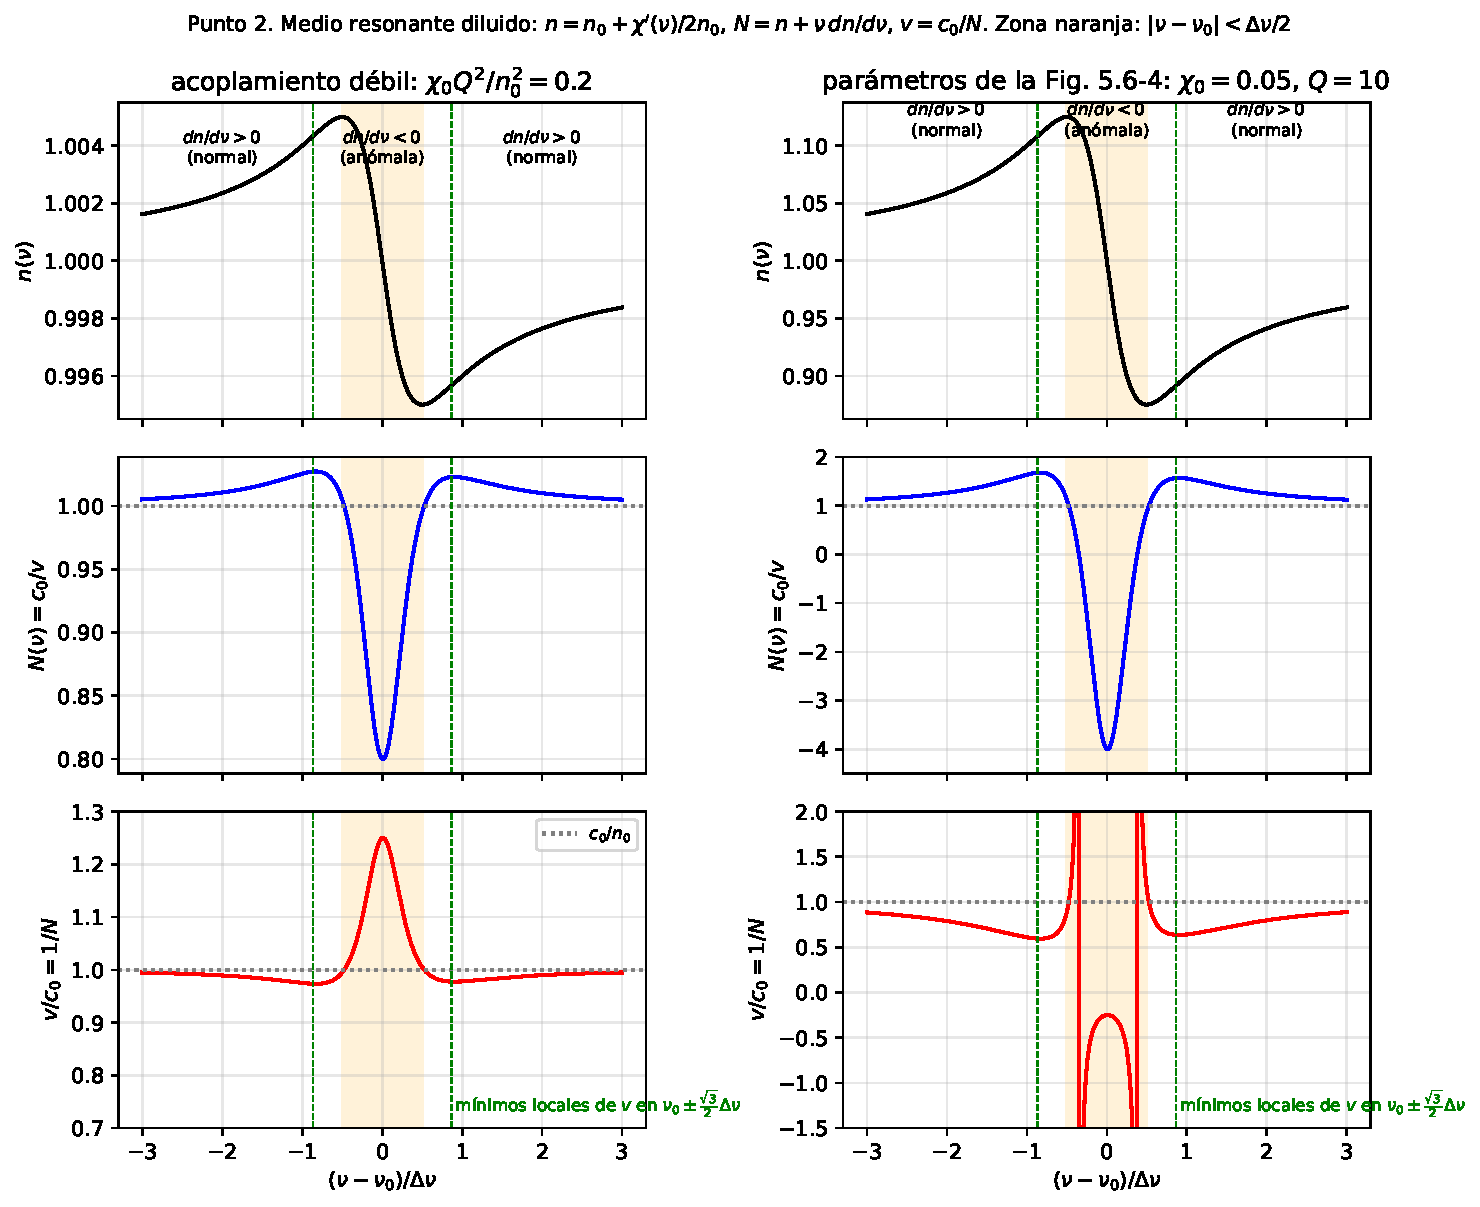
\includegraphics[width=\textwidth]{punto2_velocidad_grupo}
\caption{Índice $n$, índice de grupo $N$ y velocidad de grupo $v/c_0$ en función de la
desintonía normalizada, ecs.~\eqref{eq:n_res} y \eqref{eq:N_exacta}, con $n_0=1$. Izquierda:
acoplamiento débil ($\chi_0Q^2/n_0^2=0.2$), que es el ``dibujo a mano alzada'' genérico.
Derecha: los parámetros de la Fig.~5.6-4 del libro ($\chi_0=0.05$ y $\Delta\nu/\nu_0=0.1$,
es decir $Q=10$; p.~187), con los que \eqref{eq:N_res} da $N(\nu_0)=-4$ y $v$ se hace negativa
(en la figura del libro esa zona queda fuera de escala y aparece sombreada como no significativa).
Este panel ilustra la forma de las curvas, pero excede la hipótesis de medio diluido, pues
el máximo de $|\chi''|$ es $\chi_0Q=0.5$; con el modelo de Lorentz completo (5.5-19) resulta $N(\nu_0)\approx-3.6$. La franja naranja es $|\nu-\nu_0|<\Delta\nu/2$ (dispersión
anómala en el sentido clásico $dn/d\nu<0$); las líneas verdes marcan
$\nu_0\pm\tfrac{\sqrt3}{2}\Delta\nu$, donde $v$ tiene mínimos locales.}
\label{fig:p2}
\end{figure}

\subsection*{Regiones de dispersión normal y anómala}

Hay dos criterios en uso y conviene distinguirlos.

\paragraph{Criterio clásico (signo de $dn/d\nu$).} Dispersión \emph{normal} cuando el índice
crece con la frecuencia ($dn/d\nu>0$, equivalentemente $dn/d\lambda<0$, como en el vidrio en el
visible) y \emph{anómala} cuando decrece. De \eqref{eq:n_res}, $dn/d\nu\propto-(a^2-\delta^2)$,
así que:
\[
\text{normal: } |\nu-\nu_0|>\tfrac12\Delta\nu,\qquad
\text{anómala: } |\nu-\nu_0|<\tfrac12\Delta\nu\ (\text{el interior de la línea de absorción}).
\]
En la curva de $v$: en la región anómala $N<n_0$ y $v>c_0/n_0$ (luz rápida; si $N(\nu_0)>0$, $v$ tiene su pico en $\nu_0$);
en las regiones normales $N>n_0$ y $v<c_0/n_0$ (luz lenta, mínimos en
$\nu_0\pm\tfrac{\sqrt3}{2}\Delta\nu$), con $v\to c_0/n_0$ lejos de la línea. La frontera entre
ambas son los puntos $v=c_0/n_0$ en $\nu_0\pm\tfrac12\Delta\nu$.

\paragraph{Criterio de dispersión de velocidad de grupo (Saleh, §5.6).} El libro llama normal a
$\Dnu=d(1/v)/d\nu=(1/c_0)\,dN/d\nu>0$ ($\Dlam<0$) y anómala a $\Dnu<0$. Como
$dN/d\delta=\dfrac{\chi_0Q^2}{n_0}\cdot\dfrac{2\delta(3a^2-\delta^2)}{(\delta^2+a^2)^3}\cdot a^2$
cambia de signo en $\delta=0$ y en $\delta=\pm\sqrt3a$:
\[
\begin{array}{ll}
\nu<\nu_0-\tfrac{\sqrt3}{2}\Delta\nu: & dN/d\nu>0 \;\text{(normal: pendiente positiva de $N$)}\\[2pt]
\nu_0-\tfrac{\sqrt3}{2}\Delta\nu<\nu<\nu_0: & dN/d\nu<0 \;\text{(anómala)}\\[2pt]
\nu_0<\nu<\nu_0+\tfrac{\sqrt3}{2}\Delta\nu: & dN/d\nu>0 \;\text{(normal)}\\[2pt]
\nu>\nu_0+\tfrac{\sqrt3}{2}\Delta\nu: & dN/d\nu<0 \;\text{(anómala)}
\end{array}
\]
Este es exactamente el comportamiento de la Fig.~5.6-4 del libro: lejos de la resonancia y por
debajo de ella (el caso del vidrio, cuyas resonancias están en el ultravioleta) la dispersión es
normal; por encima de la resonancia es anómala; y al acercarse a la línea cada una cambia de
signo. Como advierte el texto (zona sombreada de la Fig.~5.6-4), muy cerca
de $\nu_0$ el índice varía tan rápido que $N$ y $D$, definidos por una
expansión de Taylor de $\beta(\omega)$ truncada, dejan de describir bien un pulso real: ahí los
términos de orden superior lo deforman y la velocidad de grupo pierde su significado.

\paragraph{Validez de la expresión.} \eqref{eq:v_res} supone (i) medio diluido
($|\chi'|,|\chi''|\ll1$, punto 1), (ii) aproximación de resonancia $|\delta|\ll\nu_0$
(ecs.~5.5-22 a 5.5-24), (iii) $Q\gg1$ para despreciar el término $\delta/(\delta^2+a^2)$ de
\eqref{eq:N_exacta}, y (iv) ausencia de absorción en el cálculo de $v$: cerca de $\nu_0$ la
absorción $\alpha=-(2\pi\nu/n_0c_0)\chi''$ es máxima y un pulso que viaje a esa velocidad se
atenúa fuertemente, lo que en la práctica obliga a usar medios con ganancia para observar la luz
rápida o lenta.

%=====================================================================
\section{Punto 3: retardo y ensanchamiento de un pulso gaussiano de \SI{100}{ps} en \SI{1}{km} de fibra}
%=====================================================================

\emph{Un pulso gaussiano con ancho inicial $\tau_0=\SI{100}{ps}$ viaja una distancia de
\SI{1}{km} a través de una fibra óptica de sílice con las características de la Fig.~5.6-5
(p.~189). Estimar el tiempo de retardo $\tau_d$ y el ancho del pulso recibido si la longitud de
onda es a) \SI{0.8}{\um}, b) \SI{1.312}{\um}, c) \SI{1.55}{\um}.}

\subsection*{Datos de la Fig.~5.6-5}

La figura se construye con la ecuación de Sellmeier (5.5-28) y los coeficientes de la sílice
fundida de la tabla 5.5-1,
\[
n^2(\lambda)=1+\frac{0.6962\,\lambda^2}{\lambda^2-0.06840^2}
+\frac{0.4079\,\lambda^2}{\lambda^2-0.1162^2}
+\frac{0.8975\,\lambda^2}{\lambda^2-9.8962^2}\qquad(\lambda\text{ en \um}),
\]
y las definiciones $N=n-\lambda_0\,dn/d\lambda_0$ (5.6-2) y
$\Dlam=-(\lambda_0/c_0)\,d^2n/d\lambda_0^2$ (5.6-7). En lugar de leer las curvas a ojo se
evaluaron numéricamente (función \texttt{dispersion\_silice} del programa del punto 4, que
reproduce la figura; véase la Fig.~\ref{fig:p3}). La lectura gráfica da
$N\approx1.467$, $1.462$ y $1.463$ y $\Dlam\approx-110$, $\approx0$ y $\approx+22$ \pskmnm, compatible
con los valores calculados de la Tabla~\ref{tab:p3_sellmeier}, salvo que en \SI{1.312}{\um} la
Sellmeier no da exactamente cero, como se explica a continuación.

\begin{table}[H]
\centering
\caption{Parámetros de la sílice fundida (Sellmeier, tabla 5.5-1) en las tres longitudes de
onda. $\Dnu=-\Dlam\lambda_0^2/c_0$ (de $\Dlam\,d\lambda=\Dnu\,d\nu$, p.~186).}
\label{tab:p3_sellmeier}
\begin{tabular}{S[table-format=1.3] S[table-format=1.5] S[table-format=1.5] S[table-format=+3.2] S[table-format=+1.3e-2]}
\toprule
{$\lambda_0$ (\um)} & {$n$} & {$N$} & {$\Dlam$ (\pskmnm)} & {$\Dnu$ (\si{s^2/m})}\\
\midrule
0.800 & 1.45331 & 1.46713 & -106.36 & +2.271e-25\\
1.312 & 1.44678 & 1.46164 & +3.78   & -2.172e-26\\
1.550 & 1.44402 & 1.46259 & +21.92  & -1.757e-25\\
\bottomrule
\end{tabular}
\end{table}

El cero de dispersión de la sílice \emph{masiva} según esta Sellmeier está en
$\lambda_0=\SI{1.273}{\um}$ (el libro cita \SI{1.276}{\um}); el valor de \SI{1.312}{\um} que
menciona el ejemplo 5.6-1 corresponde a las fibras dopadas (p.~189); en una fibra el cero se
desplaza por el dopaje y por la dispersión de guía (§9.3). Para el inciso b) se toma entonces $\Dlam\approx0$ como pretende el enunciado, y se anota
entre paréntesis el valor residual de la sílice masiva, $+3.8$ \pskmnm, que en cualquier caso es
treinta veces menor que en a).

\subsection*{Tiempo de retardo}

El pulso viaja a la velocidad de grupo $v=c_0/N$ (5.6-2), de modo que el retardo de grupo es
\[
\tau_d=\frac{z}{v}=\frac{N\,z}{c_0}=\frac{N\times\SI{1000}{m}}{\SI{2.998e8}{m/s}}
=N\times\SI{3.3356}{\micro\second}.
\]
\begin{center}
\begin{tabular}{lS[table-format=1.5]S[table-format=1.4]}
\toprule
caso & {$N$} & {$\tau_d$ (\si{\micro\second})}\\
\midrule
a) \SI{0.8}{\um}   & 1.46713 & 4.8938\\
b) \SI{1.312}{\um} & 1.46164 & 4.8755\\
c) \SI{1.55}{\um}  & 1.46259 & 4.8787\\
\bottomrule
\end{tabular}
\end{center}
El retardo es de unos \SI{4.88}{\micro\second} en los tres casos; difiere entre longitudes de
onda en menos de \SI{20}{ns} (el \SI{0.4}{\percent}), porque el índice de grupo de la sílice es
casi plano entre \SI{0.8}{} y \SI{1.6}{\um} (tiene su mínimo en el cero de dispersión).

\subsection*{Ancho del pulso recibido}

\paragraph{Definición del ancho.} Se toma la envolvente gaussiana en la forma de Saleh (§22.3) y
del punto 4, $A(0,t)=\exp(-t^2/\tau_0^2)$, con $\tau_0$ la semianchura a $1/e$ de la amplitud
(la intensidad $|A|^2$ tiene semianchura $\tau_0/\sqrt2$ y anchura total a media altura
$\sqrt{2\ln2}\,\tau_0=1.18\,\tau_0$). Su espectro es también gaussiano,
$A(0,\nu)=\sqrt\pi\,\tau_0\exp(-\pi^2\tau_0^2\nu^2)$, con semianchura a $1/e$
$\sigma_\nu=1/\pi\tau_0$.

\paragraph{Solución exacta.} En el punto 4 se demuestra que la ecuación de la envolvente
$\partial A/\partial z=j(\Dnu/4\pi)\,\partial^2A/\partial t^2$ propaga un pulso gaussiano
conservando su forma, con semianchura
\begin{equation}
\tau(z)=\tau_0\sqrt{1+\left(\frac{z}{z_0}\right)^2},\qquad
z_0=\frac{\pi\tau_0^2}{|\Dnu|},
\label{eq:tau_z}
\end{equation}
donde $z_0$ es la \emph{distancia de dispersión}: a $z=z_0$ el ancho se ha multiplicado por
$\sqrt2$ (son las ecs.~22.3-10 y 22.3-12 del libro, p.~964, con $D_\nu=2\pi\beta''$, es
decir $z_0=\tau_0^2/2|\beta''|$). Equivalentemente, $\tau^2(z)=\tau_0^2+\sigma_\tau^2$ con
$\sigma_\tau=|\Dnu|\,z/\pi\tau_0=|\Dnu|\,\sigma_\nu\,z$: el ensanchamiento añadido es
justamente la estimación (5.6-5) del libro, $\sigma_\tau=|\Dnu|\sigma_\nu z$, y se combina en
cuadratura con el ancho inicial.

\paragraph{Estimación con (5.6-8).} En términos de longitud de onda, $\sigma_\tau=|\Dlam|\sigma_\lambda z$
con $\sigma_\lambda=\lambda_0^2\sigma_\nu/c_0$. Para $\tau_0=\SI{100}{ps}$,
$\sigma_\nu=1/(\pi\times\SI{100}{ps})=\SI{3.18}{GHz}$, un espectro extraordinariamente estrecho:
$\sigma_\lambda=\SI{6.8e-3}{nm}$ en \SI{0.8}{\um} y \SI{2.6e-2}{nm} en \SI{1.55}{\um}.

\begin{table}[H]
\centering
\caption{Ensanchamiento del pulso de $\tau_0=\SI{100}{ps}$ tras $z=\SI{1}{km}$.}
\label{tab:p3_anchos}
\begin{tabular}{l S[table-format=1.2e-2] S[table-format=4.0] S[table-format=1.3] S[table-format=3.4] S[table-format=1.1e-1]}
\toprule
caso & {$\sigma_\lambda$ (nm)} & {$z_0$ (km)} & {$\sigma_\tau$ (ps)} & {$\tau(\SI{1}{km})$ (ps)} & {$\tau/\tau_0-1$}\\
\midrule
a) \SI{0.8}{\um}, $\Dlam=-106$   & 6.8e-3 & 138  & 0.723 & 100.0026 & 2.6e-5\\
b) \SI{1.312}{\um}, $\Dlam\approx0$ (+3.8) & 1.8e-2 & {($1447$)} & {0 (0.069)} & {100.0000} & {$<10^{-6}$}\\
c) \SI{1.55}{\um}, $\Dlam=+21.9$ & 2.6e-2 & 179  & 0.559 & 100.0016 & 1.6e-5\\
\bottomrule
\end{tabular}
\end{table}

\paragraph{Resultado.} Con $\tau_0=\SI{100}{ps}$ la distancia de dispersión es de más de
\SI{100}{km} en los tres casos, así que en \SI{1}{km} ($z\ll z_0$) el pulso llega con su ancho
prácticamente intacto: el ensanchamiento añadido es de \SI{0.72}{ps} en \SI{0.8}{\um}, nulo (del
orden de \SI{0.07}{ps} por la dispersión residual) en \SI{1.312}{\um} y \SI{0.56}{ps} en
\SI{1.55}{\um}, lo que al combinarse en cuadratura con \SI{100}{ps} cambia el ancho en menos de
tres partes en $10^5$. El retardo, en cambio, sí es apreciable: $\tau_d\approx\SI{4.88}{\micro\second}$.
El signo de $\Dlam$ no afecta la magnitud del ensanchamiento, pero sí el chirp: en
\SI{0.8}{\um} (dispersión normal) las componentes rojas del pulso adelantan a las azules, en
\SI{1.55}{\um} (anómala) ocurre lo contrario (Fig.~5.6-3).

\paragraph{Complemento: por qué \SI{100}{ps} es ``largo''.} Como $\sigma_\tau\propto1/\tau_0$, la
dispersión solo importa cuando $\tau_0\lesssim\sqrt{|\Dnu|z/\pi}$, que para \SI{1}{km} de
sílice es $\approx\SI{8.5}{ps}$ en \SI{0.8}{\um}. Un pulso de \SI{100}{fs} en la misma fibra
tendría $z_0=\SI{0.14}{m}$, $\SI{1.4}{m}$ y $\SI{0.18}{m}$ y saldría con \SI{723}{ps},
\SI{69}{ps} y \SI{559}{ps} de ancho, respectivamente. En \SI{1.312}{\um} se usó el valor residual
$+3.8$ \pskmnm; ahí pesa además la dispersión de orden superior, y con la fase completa de la
Sellmeier resulta $\approx\SI{67}{ps}$. Esa dependencia es la que se explora en el
punto 4 con pulsos de \SI{10}{ps} y \SI{1}{ps}.

\begin{figure}[H]
\centering
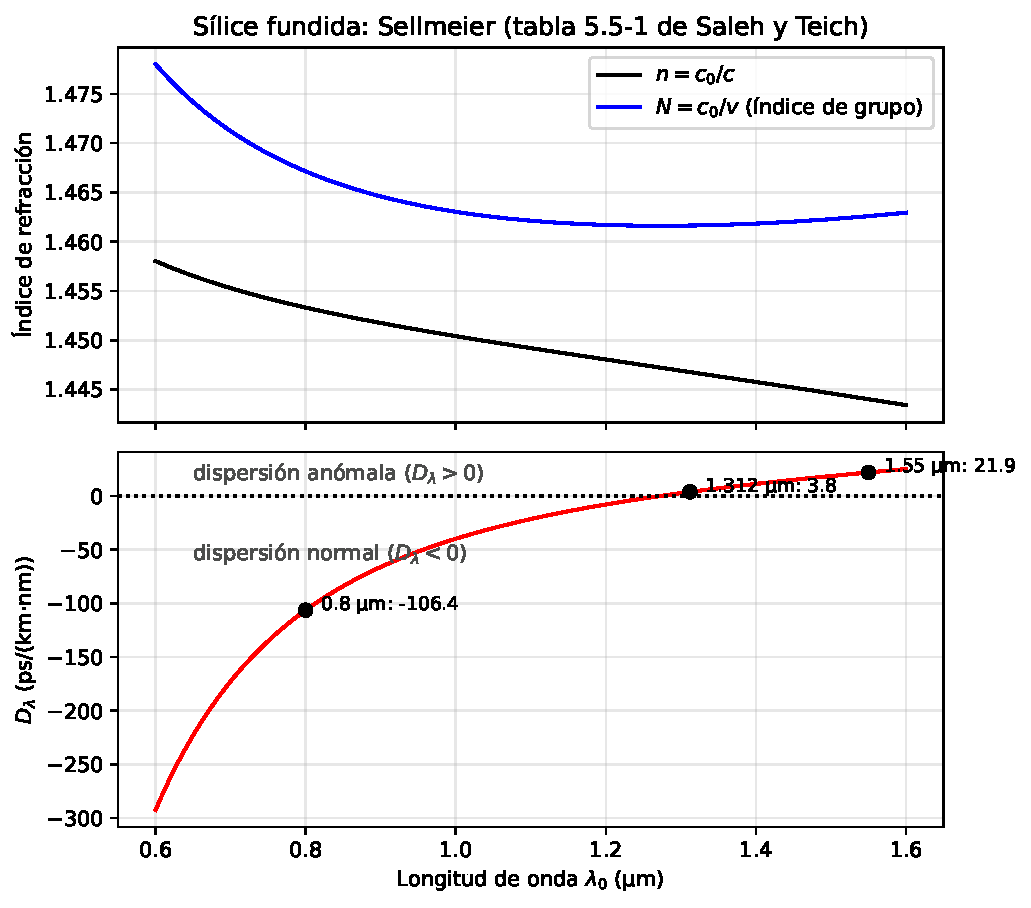
\includegraphics[width=0.8\textwidth]{punto3_fig_5_6_5}
\caption{Reproducción de la Fig.~5.6-5 con la Sellmeier de la tabla 5.5-1 (programa del punto
4). Puntos: las tres longitudes de onda del enunciado.}
\label{fig:p3}
\end{figure}

%=====================================================================
\section{Punto 4: programa en MATLAB para la ecuación de la envolvente}
%=====================================================================

\emph{Escribir un programa en MATLAB que resuelva la ecuación
$\dfrac{\partial A}{\partial z}=j\dfrac{\Dnu}{4\pi}\dfrac{\partial^2A}{\partial t^2}$
utilizando el método $A(z,t)=F^{-1}\!\left[H(\nu,z)\,F[A(0,z)]\right]$. Probar el programa
graficando la amplitud del pulso versus tiempo para $z=0$, $0.2$, $0.4$, $0.6$ y \SI{1}{km}, con
pulso inicial gaussiano: a) ancho \SI{10}{ps}, $\lambda_0=\SI{0.8}{\um}$; b) \SI{10}{ps},
\SI{1.55}{\um}; c) \SI{1}{ps}, \SI{0.8}{\um}; d) \SI{1}{ps}, \SI{1.55}{\um}. Utilice la
Fig.~5.6-5 para calcular la dispersión.}

\subsection*{Origen de la ecuación y función de transferencia}

Para un pulso $U(z,t)=A(z,t)\exp[j(\omega_0t-\beta_0z)]$ en un medio con constante de propagación
$\beta(\omega)\approx\beta_0+\beta'\Omega+\tfrac12\beta''\Omega^2$ ($\Omega=\omega-\omega_0$),
cada componente de Fourier de la envolvente, de frecuencia $\nu=\Omega/2\pi$, se propaga como
$\exp\{-j[\beta'\Omega+\tfrac12\beta''\Omega^2]z\}$. En el marco que viaja con el pulso a la
velocidad de grupo ($t\to t-z/v$) solo queda el término cuadrático, y con
$\Dnu=2\pi\beta''$ (5.6-4) y $\Omega=2\pi\nu$,
\[
A(z,\nu)=H(\nu,z)\,A(0,\nu),\qquad
\boxed{\,H(\nu,z)=\exp\!\left(-j\pi\Dnu\,\nu^2z\right)\,}.
\]
Esta es la solución de la ecuación del enunciado: con la convención
$F[f](\nu)=\int f\,e^{-j2\pi\nu t}\dd t$ (A.1-2), $\partial^2/\partial t^2\to(j2\pi\nu)^2=-4\pi^2\nu^2$, y
\[
\frac{\partial A(z,\nu)}{\partial z}=j\frac{\Dnu}{4\pi}\left(-4\pi^2\nu^2\right)A(z,\nu)
=-j\pi\Dnu\nu^2A(z,\nu)
\;\Longrightarrow\; A(z,\nu)=A(0,\nu)\,e^{-j\pi\Dnu\nu^2z}.
\]
El medio actúa sobre la envolvente como un filtro lineal de fase pura (``all-pass''): no cambia
el espectro de potencia $|A(\nu)|^2$, solo le imprime una fase cuadrática. El algoritmo es
entonces
\[
A(z,t)=F^{-1}\!\left[e^{-j\pi\Dnu\nu^2z}\,F[A(0,t)]\right],
\]
y en MATLAB $F$ y $F^{-1}$ son \texttt{fft} e \texttt{ifft}, que usan la misma convención de
signos que el libro ($e^{-j2\pi kn/N}$ en la transformada directa).

\paragraph{Solución analítica de control.} Para $A(0,t)=\exp(-t^2/\tau_0^2)$,
$F[A]=\sqrt\pi\tau_0\exp(-\pi^2\tau_0^2\nu^2)$, y
\[
A(z,\nu)=\sqrt\pi\tau_0\exp\!\left[-\pi^2\nu^2\left(\tau_0^2+j\frac{\Dnu z}{\pi}\right)\right]
\;\Longrightarrow\;
A(z,t)=\frac{1}{\sqrt{1+jz/z_0}}\exp\!\left[-\frac{t^2}{\tau_0^2\,(1+jz/z_0)}\right],
\quad z_0=\frac{\pi\tau_0^2}{\Dnu},
\]
que se obtiene por la transformada inversa de una gaussiana de ``anchura compleja''
$\tau_0^2(1+jz/z_0)$. Aquí $z_0$ lleva el signo de $\Dnu$, como en (22.3-12); las distancias de
dispersión que se tabulan son su magnitud, la de \eqref{eq:tau_z}. Separando el exponente, $\dfrac{1}{1+jz/z_0}=\dfrac{1-jz/z_0}{1+(z/z_0)^2}$:
\[
|A(z,t)|=\frac{1}{[1+(z/z_0)^2]^{1/4}}\exp\!\left[-\frac{t^2}{\tau^2(z)}\right],\qquad
\tau(z)=\tau_0\sqrt{1+(z/z_0)^2},\qquad
\arg A=\frac{z/z_0}{1+(z/z_0)^2}\frac{t^2}{\tau_0^2}+\text{const}.
\]
El pulso sigue siendo gaussiano, se ensancha según \eqref{eq:tau_z}, su amplitud máxima cae como
$[1+(z/z_0)^2]^{-1/4}$ (la energía $\int|A|^2dt$ se conserva) y adquiere un chirp lineal:
la frecuencia instantánea $\nu_i-\nu_0=\frac{1}{2\pi}\frac{d\arg A}{dt}\propto\Dnu\,t$ crece con $t$
si $\Dnu>0$ (dispersión normal, \SI{0.8}{\um}: la cola del pulso es más azul) y decrece si
$\Dnu<0$ (anómala, \SI{1.55}{\um}). El valor absoluto $|A|$ es el mismo para $\pm\Dnu$.

\subsection*{Parámetros de dispersión}

$\Dnu$ se obtiene de la Fig.~5.6-5 a través de la Sellmeier (Tabla~\ref{tab:p3_sellmeier}):
$\Dnu=-\Dlam\lambda_0^2/c_0=+\SI{2.271e-25}{s^2/m}$ en \SI{0.8}{\um} y
$\SI{-1.757e-25}{s^2/m}$ en \SI{1.55}{\um} (en unidades de fibra,
$\beta''=\Dnu/2\pi=+36.1$ y $-28.0$ \si{ps^2/km}). Con ellos las distancias de dispersión son
\begin{gather*}
z_0(\SI{10}{ps},\SI{0.8}{\um})=\SI{1.38}{km},\qquad
z_0(\SI{10}{ps},\SI{1.55}{\um})=\SI{1.79}{km},\\
z_0(\SI{1}{ps},\SI{0.8}{\um})=\SI{13.8}{m},\qquad
z_0(\SI{1}{ps},\SI{1.55}{\um})=\SI{17.9}{m},
\end{gather*}
que anticipan lo que se verá: ensanchamiento moderado ($z\sim z_0$) para \SI{10}{ps} y enorme
($z\approx56$--$72\,z_0$) para \SI{1}{ps}.

\subsection*{El programa}

El código completo está en el Apéndice~\ref{ap:codigo} (archivo
\texttt{punto4\_pulso\_dispersion.m}). Sus pasos son:
\begin{enumerate}
\item \texttt{dispersion\_silice(lam)}: evalúa la Sellmeier y, por diferencias finitas centradas
($h=\SI{0.1}{nm}$), $dn/d\lambda$ y $d^2n/d\lambda^2$; devuelve $n$, $N$, $\Dlam$ y $\Dnu$.
Con ella reproduce la Fig.~5.6-5 (Fig.~\ref{fig:p3}).
\item Para cada caso construye una malla temporal de $N_t=2^{16}$ puntos con ventana
$T=24\,\tau(\SI{1}{km})$, de modo que el pulso más ancho cabe holgadamente (sin aliasing
temporal) y el inicial queda bien muestreado (paso $\Delta t=T/N_t$: \SI{4.5}{fs} y \SI{4.2}{fs} para los
casos de \SI{10}{ps} y \SI{26.5}{fs} y \SI{20.5}{fs} para los de \SI{1}{ps}; el ancho de banda de Nyquist
$1/2\Delta t\geq\SI{18.9}{THz}$ supera con creces el espectro del pulso, $\sigma_\nu\leq\SI{0.32}{THz}$).
\item Calcula $A(0,\nu)$ con \texttt{fftshift(fft(ifftshift(A0)))} (eje de frecuencias centrado
en cero, $\nu_k=k/N_t\Delta t$), multiplica por $H(\nu,z)$ y vuelve al tiempo con
\texttt{fftshift(ifft(ifftshift($\cdot$)))}, para cada $z$ de la lista.
\item Grafica $|A(z,t)|$, mide la semianchura a $1/e$ del resultado numérico por interpolación y
la compara con \eqref{eq:tau_z}.
\end{enumerate}
Se ejecuta con \texttt{punto4\_pulso\_dispersion} desde la carpeta del taller. El mismo algoritmo
se escribió línea a línea en Python (\texttt{punto4\_pulso\_dispersion\_py.py}, con
\texttt{numpy.fft}). Las figuras y la tabla de esta sección provienen de esa réplica, porque el
programa de MATLAB no se pudo ejecutar en esta máquina por un error de licencia (5201).

\subsection*{Resultados}

\begin{figure}[H]
\centering
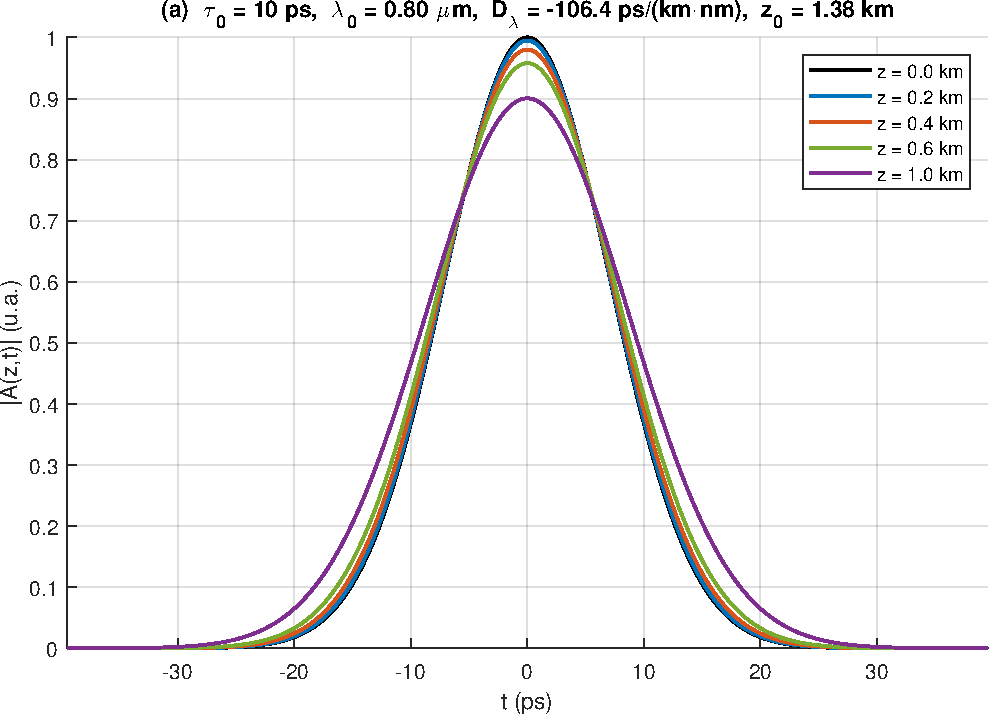
\includegraphics[width=0.49\textwidth]{punto4_caso_a}\hfill
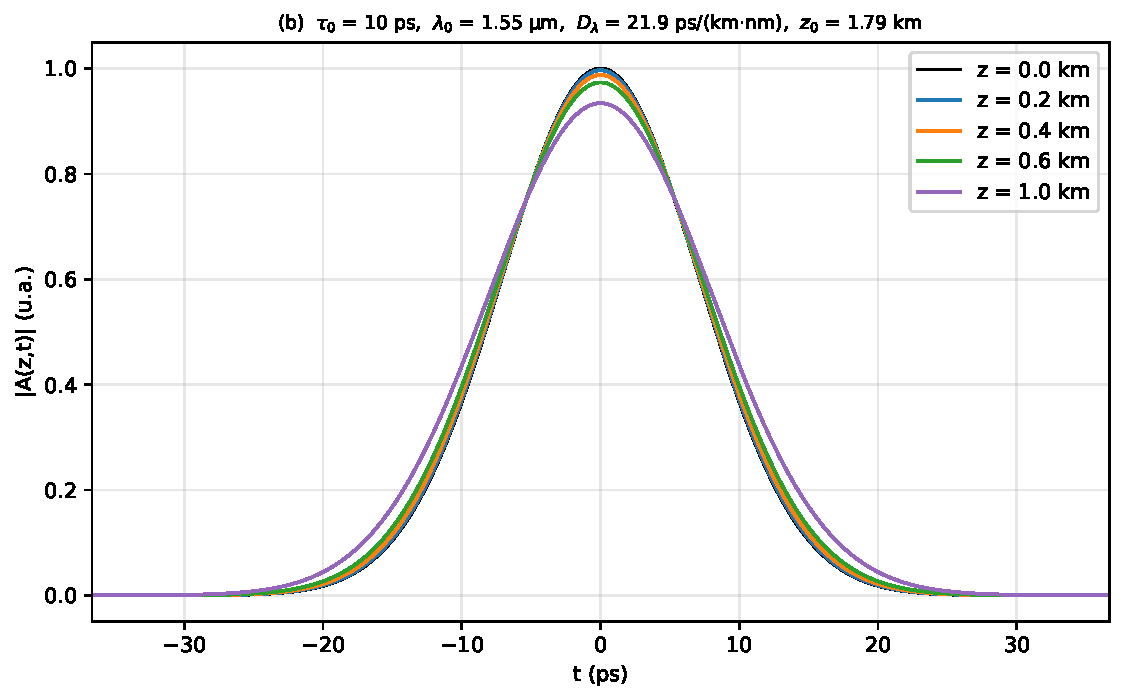
\includegraphics[width=0.49\textwidth]{punto4_caso_b}\\[4pt]
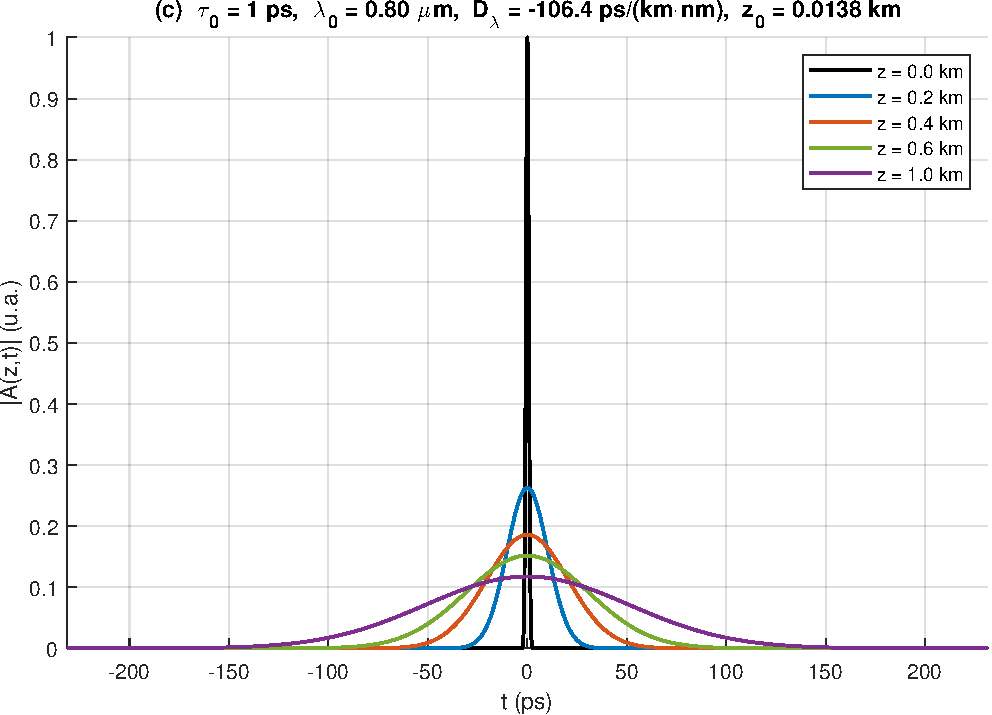
\includegraphics[width=0.49\textwidth]{punto4_caso_c}\hfill
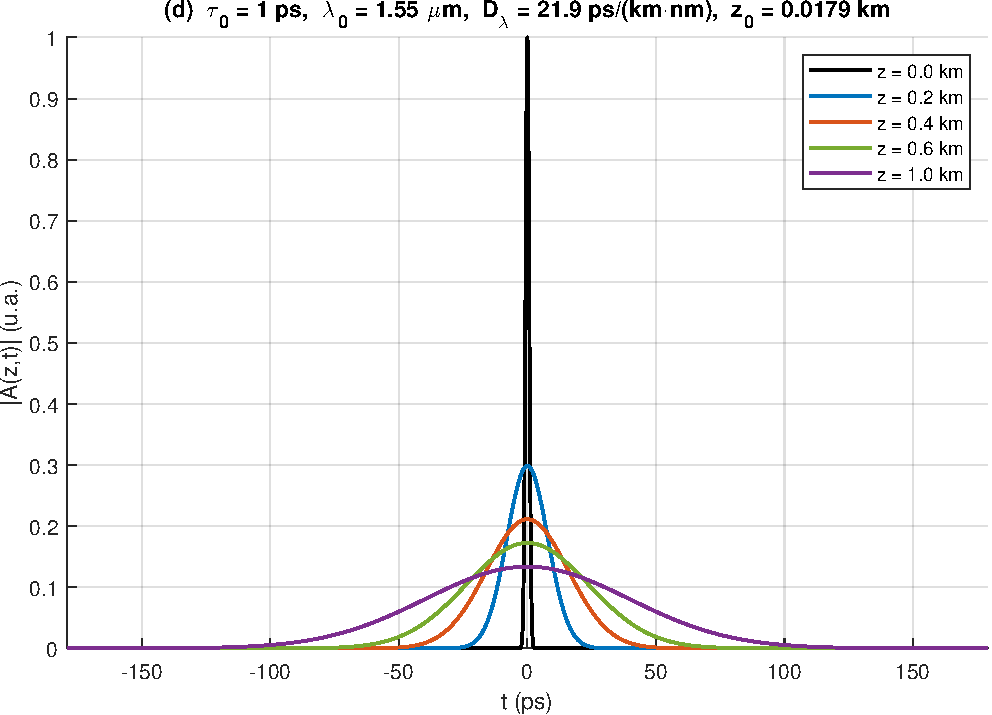
\includegraphics[width=0.49\textwidth]{punto4_caso_d}
\caption{$|A(z,t)|$ para $z=0$, $0.2$, $0.4$, $0.6$ y \SI{1}{km} en los cuatro casos. Arriba:
$\tau_0=\SI{10}{ps}$ en \SI{0.8}{\um} (a) y \SI{1.55}{\um} (b). Abajo: $\tau_0=\SI{1}{ps}$ en
\SI{0.8}{\um} (c) y \SI{1.55}{\um} (d). Obsérvese la escala temporal: en (c) y (d) el pulso
inicial de \SI{1}{ps} es la aguja central.}
\label{fig:p4}
\end{figure}

\begin{table}[H]
\centering
\caption{Semianchura a $1/e$ de $|A|$, en ps, de la solución numérica (FFT) y de la analítica
\eqref{eq:tau_z}. Coinciden en todas las cifras mostradas.}
\label{tab:p4}
\begin{tabular}{l S S S[table-format=2.2] S[table-format=2.2] S[table-format=2.2] S[table-format=2.2] S[table-format=2.2]}
\toprule
caso & {$\tau_0$ (ps)} & {$z_0$ (km)} & {$z=0$} & {\SI{0.2}{km}} & {\SI{0.4}{km}} & {\SI{0.6}{km}} & {\SI{1}{km}}\\
\midrule
a) \SI{0.8}{\um}  & 10 & 1.384 & 10.00 & 10.10 & 10.41 & 10.90 & 12.34\\
b) \SI{1.55}{\um} & 10 & 1.788 & 10.00 & 10.06 & 10.25 & 10.55 & 11.46\\
c) \SI{0.8}{\um}  & 1  & 0.0138 & 1.00 & 14.49 & 28.93 & 43.38 & 72.28\\
d) \SI{1.55}{\um} & 1  & 0.0179 & 1.00 & 11.23 & 22.39 & 33.57 & 55.93\\
\bottomrule
\end{tabular}
\end{table}

\begin{figure}[H]
\centering
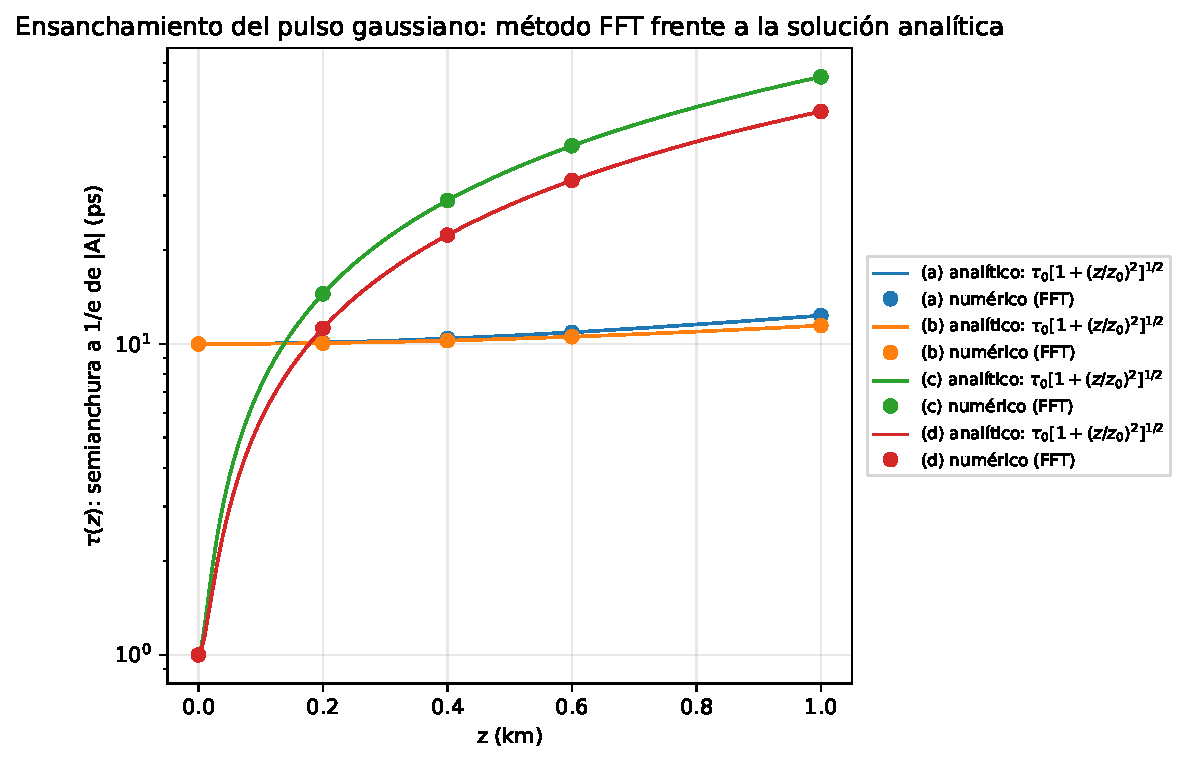
\includegraphics[width=0.85\textwidth]{punto4_anchos}
\caption{Ancho del pulso frente a la distancia: puntos, medidos sobre la solución FFT; líneas,
$\tau_0[1+(z/z_0)^2]^{1/2}$. La concordancia valida el programa.}
\label{fig:p4b}
\end{figure}

\paragraph{Discusión.}
\begin{itemize}
\item \textbf{Casos a) y b) (\SI{10}{ps}).} Como $z_0$ es comparable a \SI{1}{km}, el pulso se
ensancha un \SI{23}{\percent} en \SI{0.8}{\um} y un \SI{15}{\percent} en \SI{1.55}{\um}, y su
amplitud máxima cae a $[1+(z/z_0)^2]^{-1/4}=0.90$ y $0.93$. El ensanchamiento es menor en
\SI{1.55}{\um} porque $|\Dnu|$ es menor ahí (la dispersión anómala de la sílice en
\SI{1.55}{\um} es más débil en valor absoluto que la normal en \SI{0.8}{\um}).
\item \textbf{Casos c) y d) (\SI{1}{ps}).} Al reducir $\tau_0$ diez veces, $z_0$ cae cien veces
($z_0\propto\tau_0^2$) y a \SI{1}{km} el pulso es $\approx z/z_0$ veces más ancho: \SI{72}{ps} y
\SI{56}{ps}. En este régimen $\tau(z)\approx|\Dnu|z/\pi\tau_0$: el ancho final es
\emph{inversamente} proporcional al inicial, porque un pulso más corto tiene un espectro más
ancho y la dispersión separa más sus componentes. La amplitud cae a $0.12$ y $0.13$.
\item \textbf{Signo de la dispersión.} Las curvas de $|A|$ de a) y b) tienen la misma forma salvo
por la magnitud de $\Dnu$; la diferencia entre dispersión normal y anómala está en la fase
(chirp de signo opuesto), que no se ve en $|A|$. Esto es lo que permite compensar la dispersión
de un tramo de fibra con otro de signo contrario.
\item \textbf{Consistencia con el punto 3.} Para $\tau_0=\SI{100}{ps}$ la fórmula \eqref{eq:tau_z} da
$z_0=\SI{138}{km}$ y $\tau(\SI{1}{km})=\SI{100.003}{ps}$, como se calculó allí.
\end{itemize}

%=====================================================================
\section{Punto 5: Problema 6.1-8, retardadores de onda en tándem}
%=====================================================================

\emph{Escriba las matrices de Jones de: (a) un retardador de $\pi/2$ con eje rápido en $x$; (b)
un retardador de $\pi$ con eje rápido a $45^\circ$ de $x$; (c) un retardador de $\pi/2$ con eje
rápido en $y$. Si los tres se colocan en tándem, (c) tras (b) tras (a), demuestre que el
dispositivo resultante introduce una rotación de $90^\circ$. ¿Qué ocurre si se invierte el
orden?} (p.~241.)

\subsection*{Matrices de cada elemento}

Un retardador con eje rápido en $x$ y retardo $\Gamma$ deja la componente $x$ intacta y
retrasa la $y$ en la fase $\Gamma$ (6.1-19): $\Tm=\mathrm{diag}(1,e^{-j\Gamma})$. Para un eje
rápido que forma un ángulo $\theta$ con $x$ se usa la transformación de coordenadas (6.1-24),
$\Tm=\Rm(-\theta)\,\Tm'\,\Rm(\theta)$, con
$\Rm(\theta)=\begin{bmatrix}\cos\theta&\sin\theta\\-\sin\theta&\cos\theta\end{bmatrix}$ (6.1-22).

\begin{enumerate}
\item[(a)] $\Gamma=\pi/2$, eje rápido $x$:
\[
\Tm_a=\begin{bmatrix}1&0\\0&e^{-j\pi/2}\end{bmatrix}=\begin{bmatrix}1&0\\0&-j\end{bmatrix}.
\]
\item[(b)] $\Gamma=\pi$, eje rápido a $\theta=45^\circ$. En el sistema rotado,
$\Tm'_b=\mathrm{diag}(1,e^{-j\pi})=\mathrm{diag}(1,-1)$. En general,
\[
\Rm(-\theta)\begin{bmatrix}1&0\\0&-1\end{bmatrix}\Rm(\theta)
=\begin{bmatrix}\cos\theta&-\sin\theta\\ \sin\theta&\cos\theta\end{bmatrix}
\begin{bmatrix}\cos\theta&\sin\theta\\ \sin\theta&-\cos\theta\end{bmatrix}
=\begin{bmatrix}\cos2\theta&\sin2\theta\\ \sin2\theta&-\cos2\theta\end{bmatrix},
\]
y con $\theta=45^\circ$:
\[
\Tm_b=\begin{bmatrix}0&1\\1&0\end{bmatrix}.
\]
(Comprobación: intercambia $x$ e $y$, que es lo que hace una lámina de media onda a $45^\circ$;
la Fig.~6.1-8(b) muestra el caso equivalente.)
\item[(c)] $\Gamma=\pi/2$, eje rápido $y$: ahora la componente retrasada es la $x$,
\[
\Tm_c=\begin{bmatrix}e^{-j\pi/2}&0\\0&1\end{bmatrix}=\begin{bmatrix}-j&0\\0&1\end{bmatrix}
\]
(es $\Tm_a$ con $\theta=90^\circ$ en (6.1-24), o bien $e^{-j\pi/2}\,\mathrm{diag}(1,e^{+j\pi/2})$:
salvo una fase global, un retardo de $-\pi/2$ en $y$).
\end{enumerate}

\subsection*{Los tres en tándem}

La luz atraviesa primero (a), luego (b) y por último (c); la matriz del primer elemento va a la
derecha (p.~207):
\[
\Tm=\Tm_c\Tm_b\Tm_a
=\begin{bmatrix}-j&0\\0&1\end{bmatrix}
\begin{bmatrix}0&1\\1&0\end{bmatrix}
\begin{bmatrix}1&0\\0&-j\end{bmatrix}
=\begin{bmatrix}-j&0\\0&1\end{bmatrix}
\begin{bmatrix}0&-j\\1&0\end{bmatrix}
=\begin{bmatrix}0&(-j)(-j)\\1&0\end{bmatrix}
=\boxed{\begin{bmatrix}0&-1\\1&0\end{bmatrix}}.
\]
Comparando con la matriz del rotador de polarización (6.1-20),
$\begin{bmatrix}\cos\theta&-\sin\theta\\ \sin\theta&\cos\theta\end{bmatrix}$, se ve que
$\Tm$ es exactamente un rotador con $\theta=+90^\circ$, sin siquiera una fase global.
Sobre una onda linealmente polarizada a un ángulo $\varphi$:
\[
\Tm\begin{bmatrix}\cos\varphi\\ \sin\varphi\end{bmatrix}
=\begin{bmatrix}-\sin\varphi\\ \cos\varphi\end{bmatrix}
=\begin{bmatrix}\cos(\varphi+90^\circ)\\ \sin(\varphi+90^\circ)\end{bmatrix},
\]
una polarización lineal girada $90^\circ$ \emph{cualquiera que sea} $\varphi$. Esto distingue al
dispositivo de una sola lámina de media onda, que también gira la polarización lineal pero en un
ángulo $2\theta$ que depende de la orientación de entrada (problema 6.1-7), y que no conserva la
helicidad de la luz circular. Aquí, en cambio, un estado circular derecho
$\tfrac{1}{\sqrt2}[1,\,j]^T$ se transforma en $\tfrac{1}{\sqrt2}[-j,\,1]^T=-j\cdot\tfrac{1}{\sqrt2}[1,\,j]^T$:
sigue siendo circular derecho (los modos normales del rotador son las polarizaciones circulares,
ejercicio 6.1-4).

La interpretación física es la de la Fig.~6.1-8: (a) convierte la luz lineal en elíptica
(circular si entra a $45^\circ$), (b) invierte la helicidad de esa elipse y la refleja respecto al
eje a $45^\circ$, y (c) le suma otros $\pi/2$ a la fase relativa, que pasa de $+\pi/2$ a $\pi$. La luz vuelve a ser
lineal, y ese signo menos convierte la reflexión respecto al eje a $45^\circ$ en una rotación de
$90^\circ$.

\subsection*{Orden invertido}

Si la luz atraviesa (c), luego (b) y luego (a):
\[
\Tm'=\Tm_a\Tm_b\Tm_c
=\begin{bmatrix}1&0\\0&-j\end{bmatrix}
\begin{bmatrix}0&1\\1&0\end{bmatrix}
\begin{bmatrix}-j&0\\0&1\end{bmatrix}
=\begin{bmatrix}1&0\\0&-j\end{bmatrix}
\begin{bmatrix}0&1\\-j&0\end{bmatrix}
=\begin{bmatrix}0&1\\-1&0\end{bmatrix}=-\Tm ,
\]
que es el rotador (6.1-20) con $\theta=-90^\circ$. Sobre luz lineal,
$\Tm'[\cos\varphi,\sin\varphi]^T=[\sin\varphi,-\cos\varphi]^T$: la misma recta de polarización
que antes (un giro de $-90^\circ$ y uno de $+90^\circ$ dejan la elipse en la misma orientación,
pues las elipses son invariantes ante un giro de $180^\circ$), y para luz circular la misma
helicidad. Como $\Tm'=e^{j\pi}\,\Tm$, los dos dispositivos difieren solo en una fase global de
$\pi$, que no altera el estado de polarización; solo se notaría si el haz interfiriera con otro
de referencia. En resumen: invertir el orden sigue dando una rotación de $90^\circ$ (ahora
``$-90^\circ$''), físicamente indistinguible salvo por la fase absoluta. Invertir el orden da siempre la
transpuesta, $\Tm'=\Tm^{T}$, porque la matriz de cada retardador lineal es simétrica. Lo particular
de este caso es que $\Tm$ es una rotación de $90^\circ$, que es antisimétrica, y por eso
$\Tm^T=-\Tm$.

%=====================================================================
\section{Punto 6: Problema 6.2-5, refracción en el ángulo de Brewster}
%=====================================================================

\emph{Use la condición $n_1\sec\theta_1=n_2\sec\theta_2$ y la ley de Snell,
$n_1\sin\theta_1=n_2\sin\theta_2$, para deducir (6.2-12) para el ángulo de Brewster. Muestre
también que en el ángulo de Brewster $\theta_1+\theta_2=90^\circ$, de modo que las direcciones
de las ondas reflejada y refractada son ortogonales y, por tanto, el campo eléctrico de la onda TM
refractada es paralelo a la dirección de la onda reflejada. La reflexión puede verse como un
proceso de dispersión en el que la onda refractada actúa como fuente de radiación que genera la
onda reflejada; en el ángulo de Brewster esa fuente oscila en la dirección de propagación de la
onda reflejada, así que no puede radiar y no se refleja luz TM.} (p.~241.)

\subsection*{Origen de la condición}

El coeficiente de reflexión TM (6.2-9) es
$r_y=\dfrac{n_1\sec\theta_1-n_2\sec\theta_2}{n_1\sec\theta_1+n_2\sec\theta_2}$, que se anula
cuando $n_1\sec\theta_1=n_2\sec\theta_2$, es decir,
\begin{equation}
n_1\cos\theta_2=n_2\cos\theta_1 .
\label{eq:brew}
\end{equation}
Esta condición y la ley de Snell,
\begin{equation}
n_1\sin\theta_1=n_2\sin\theta_2 ,
\label{eq:snell}
\end{equation}
deben cumplirse simultáneamente.

\subsection*{Deducción de $\theta_B=\tan^{-1}(n_2/n_1)$}

De \eqref{eq:snell} y \eqref{eq:brew} se despejan el seno y el coseno del ángulo de refracción:
\[
\sin\theta_2=\frac{n_1}{n_2}\sin\theta_1,\qquad \cos\theta_2=\frac{n_2}{n_1}\cos\theta_1 .
\]
Imponiendo $\sin^2\theta_2+\cos^2\theta_2=1$ y escribiendo $r\equiv n_2/n_1$:
\[
\frac{\sin^2\theta_1}{r^2}+r^2\cos^2\theta_1=1
\;\Longrightarrow\;
\sin^2\theta_1+r^4\left(1-\sin^2\theta_1\right)=r^2
\;\Longrightarrow\;
\sin^2\theta_1\left(1-r^4\right)=r^2\left(1-r^2\right).
\]
Como $1-r^4=(1-r^2)(1+r^2)$ y $r\neq1$ (si $n_1=n_2$ no hay reflexión),
\[
\sin^2\theta_1=\frac{r^2}{1+r^2}
\;\Longrightarrow\;
\cos^2\theta_1=\frac{1}{1+r^2}
\;\Longrightarrow\;
\tan^2\theta_1=r^2
\;\Longrightarrow\;
\boxed{\,\theta_B=\tan^{-1}\!\frac{n_2}{n_1}\,}\qquad(6.2\text{-}12).
\]
Para vidrio en aire ($n_2/n_1=1.5$) $\theta_B=56.3^\circ$; para aire desde vidrio
$\theta_B=33.7^\circ$.

\subsection*{Ortogonalidad de las ondas reflejada y refractada}

Dividiendo las dos expresiones anteriores:
\[
\tan\theta_2=\frac{\sin\theta_2}{\cos\theta_2}=\frac{(n_1/n_2)\sin\theta_1}{(n_2/n_1)\cos\theta_1}
=\left(\frac{n_1}{n_2}\right)^2\tan\theta_1 .
\]
En el ángulo de Brewster $\tan\theta_1=n_2/n_1$, luego
\[
\tan\theta_2=\left(\frac{n_1}{n_2}\right)^2\frac{n_2}{n_1}=\frac{n_1}{n_2}=\frac{1}{\tan\theta_1}=\cot\theta_1=\tan\!\left(90^\circ-\theta_1\right)
\;\Longrightarrow\;
\boxed{\,\theta_1+\theta_2=90^\circ\,}.
\]
(Lo mismo se ve directamente de \eqref{eq:brew} y \eqref{eq:snell}: al despejar $n_1/n_2$ de ambas resulta
$\sin\theta_2/\sin\theta_1=\cos\theta_1/\cos\theta_2$, es decir $\sin2\theta_1=\sin2\theta_2$, cuyas
soluciones son $\theta_1=\theta_2$, que exige $n_1=n_2$, y $\theta_1+\theta_2=90^\circ$;
sustituyendo esta última en Snell, $n_1\sin\theta_1=n_2\cos\theta_1$, que es otra vez (6.2-12).)

La onda reflejada sale con $\theta_3=\theta_1$ al otro lado de la normal y la refractada con
$\theta_2$ en el segundo medio (Fig.~\ref{fig:brewster}). El ángulo entre $\kv_3$ y $\kv_2$ es
$180^\circ-\theta_3-\theta_2=180^\circ-(\theta_1+\theta_2)=90^\circ$: \textbf{las direcciones
reflejada y refractada son ortogonales}.

\begin{figure}[H]
\centering
\begin{tikzpicture}[scale=1.0,>={Stealth[length=2.5mm]}]
  % medios
  \fill[blue!8] (-4.2,0) rectangle (4.2,-3);
  \draw[thick] (-4.2,0) -- (4.2,0);
  \node[right] at (2.6,0.35) {medio 1, $n_1$};
  \node[right] at (2.6,-0.4) {medio 2, $n_2>n_1$};
  % normal
  \draw[dashed] (0,-3) -- (0,3);
  \node[above] at (0,3) {normal};
  % ángulos: theta_B = 56.3 (n2/n1=1.5), theta_2 = 33.7
  \coordinate (O) at (0,0);
  \coordinate (Nup) at (0,1);
  \coordinate (Ndn) at (0,-1);
  \coordinate (I) at ({-3.2*sin(56.3)},{3.2*cos(56.3)});
  \coordinate (R) at ({3.2*sin(56.3)},{3.2*cos(56.3)});
  \coordinate (T) at ({3.0*sin(33.7)},{-3.0*cos(33.7)});
  % rayos
  \draw[->,very thick,red] (I) -- (O) node[pos=0.5,below left] {$\kv_1$ incidente};
  \draw[->,very thick,red] (O) -- (R) node[pos=0.8,right=3pt] {$\kv_3$ reflejada};
  \draw[->,very thick,red] (O) -- (T) node[pos=0.9,right=3pt] {$\kv_2$ refractada};
  % ángulos
  \pic[draw,angle radius=9mm,angle eccentricity=1.35,"$\theta_B$"] {angle=Nup--O--I};
  \pic[draw,angle radius=9mm,angle eccentricity=1.35,"$\theta_B$"] {angle=R--O--Nup};
  \pic[draw,angle radius=11mm,angle eccentricity=1.3,"$\theta_2$"] {angle=Ndn--O--T};
  % ángulo recto entre k2 y k3
  \coordinate (R1) at ($(O)!0.45cm!(R)$);
  \coordinate (T1) at ($(O)!0.45cm!(T)$);
  \draw (R1) -- ($(R1)+(T1)-(O)$) -- (T1);
  \node at (0.75,-0.05) {$90^\circ$};
  % campo E TM de la onda refractada (en el plano de incidencia, perpendicular a k2): paralelo a k3
  \foreach \s in {0.45,0.7}{
    \draw[<->,thick,blue!70!black] ($(O)!\s!(T)+({-0.3*sin(56.3)},{-0.3*cos(56.3)})$) -- ($(O)!\s!(T)+({0.3*sin(56.3)},{0.3*cos(56.3)})$);
  }
  \node[blue!70!black,below left] at ($(O)!0.75!(T)$) {$\Ev_2\parallel\kv_3$};
  % dipolos
  \node[blue!70!black,align=left,anchor=west] at (-4.1,-2.3) {dipolos del medio 2\\ oscilan a lo largo de $\kv_3$:\\ no radian hacia allí};
\end{tikzpicture}
\caption{Geometría en el ángulo de Brewster ($n_2/n_1=1.5$, $\theta_B=56.3^\circ$,
$\theta_2=33.7^\circ$). La onda reflejada y la refractada son perpendiculares, y el campo TM de
la onda refractada apunta justo a lo largo de la dirección reflejada.}
\label{fig:brewster}
\end{figure}

\subsection*{Por qué no se refleja la onda TM}

En la polarización TM el campo eléctrico está en el plano de incidencia y es perpendicular a
su vector de onda (onda TEM). El campo $\Ev_2$ de la onda refractada es, por tanto,
perpendicular a $\kv_2$ dentro del plano de incidencia; como $\kv_2\perp\kv_3$ y ambos
vectores están en ese plano, $\Ev_2\parallel\kv_3$.

Desde el punto de vista microscópico (modelo de Lorentz, §5.5C), la onda reflejada es la
radiación coherente de los dipolos que $\Ev_2$ induce en los átomos del medio 2, los cuales
oscilan en la dirección de $\Ev_2$. Un dipolo oscilante radia con un patrón $\propto\sin\vartheta$
(ec.~5.4-15: el campo radiado en la dirección que forma un ángulo $\vartheta$ con el eje del
dipolo es $E\propto\sin\vartheta$) y, en particular, no radia nada a lo largo de su propio eje
($\vartheta=0$). En el ángulo de Brewster ese eje coincide con la dirección $\kv_3$ de la onda
reflejada, así que la amplitud radiada en esa dirección es cero: $r_y=0$ y toda la potencia TM
se transmite. Para la polarización TE el campo es perpendicular al plano de incidencia, los
dipolos oscilan perpendicularmente a $\kv_3$ ($\vartheta=90^\circ$, radiación máxima) y
$r_x$ nunca se anula; de hecho, en el ángulo de Brewster
$r_x=\dfrac{n_1\cos\theta_1-n_2\cos\theta_2}{n_1\cos\theta_1+n_2\cos\theta_2}$ vale
$-\dfrac{n_2^2-n_1^2}{n_2^2+n_1^2}$ ($-0.385$ para vidrio), lo que explica que la luz reflejada a ese
ángulo sea puramente TE y que una lámina a incidencia de Brewster sirva como polarizador
(Fig.~6.6-2).

Un último comentario: la condición de Brewster es reversible. Si la luz viene del medio 2
(reflexión interna), el ángulo es $\theta_B'=\tan^{-1}(n_1/n_2)=90^\circ-\theta_B$, que es el
propio $\theta_2$ de antes: la ventana de Brewster (ejercicio 6.2-1) no tiene pérdidas de
reflexión para luz TM en ninguna de sus dos caras.

%=====================================================================
\section{Punto 7: Problema 6.3-2, efecto extraordinario máximo en cuarzo}
%=====================================================================

\emph{Determine la dirección de propagación en cuarzo ($n_e=1.553$, $n_o=1.544$) para la cual el
ángulo entre el vector de onda $\kv$ y el vector de Poynting $\Sv$ (que es también la dirección
de propagación del rayo) es máximo.} (p.~241.)

\subsection*{Planteamiento}

Para la onda ordinaria $\Dv\parallel\Ev$ y $\Sv\parallel\kv$ en cualquier dirección (Fig.~6.3-12a):
no hay efecto. El ángulo pedido, llamado \emph{walk-off} $\rho$, es propio de la onda
extraordinaria. Como $\Dv\perp\kv$ y $\Ev\perp\Sv$, y los cuatro vectores están en el mismo plano
(el formado por $\kv$ y el eje óptico, Fig.~6.3-8), el ángulo entre $\kv$ y $\Sv$ es igual al
ángulo entre $\Dv$ y $\Ev$.

Sea $z$ el eje óptico y $\kv=k(\sin\theta\,\yh+\cos\theta\,\zh)$ en el plano $y$--$z$, con
$\theta$ el ángulo entre $\kv$ y el eje óptico. Para la onda extraordinaria $\Dv$ está en el plano
$k$--$z$ y es perpendicular a $\kv$:
\[
\Dv=D\left(\cos\theta\,\yh-\sin\theta\,\zh\right),
\]
y la relación material en ejes principales (6.3-5), $E_y=D_y/\epsilon_0n_o^2$,
$E_z=D_z/\epsilon_0n_e^2$, da
\[
\Ev=\frac{D}{\epsilon_0}\left(\frac{\cos\theta}{n_o^2}\,\yh-\frac{\sin\theta}{n_e^2}\,\zh\right).
\]
Las direcciones de $\Dv$ y $\Ev$ medidas desde el eje $y$ tienen tangentes
$\tan\alpha_D=D_z/D_y=-\tan\theta$ y $\tan\alpha_E=E_z/E_y=-(n_o^2/n_e^2)\tan\theta$. El ángulo
entre ambos es
\[
\tan\rho=\tan(\alpha_D-\alpha_E)=\frac{\tan\alpha_D-\tan\alpha_E}{1+\tan\alpha_D\tan\alpha_E}
=\frac{-\tan\theta+(n_o^2/n_e^2)\tan\theta}{1+(n_o^2/n_e^2)\tan^2\theta}
=-\frac{(n_e^2-n_o^2)\tan\theta}{n_e^2+n_o^2\tan^2\theta}.
\]
Tomando el valor absoluto (el signo solo dice hacia qué lado se inclina $\Sv$) y multiplicando por
$\cos^2\theta$:
\begin{equation}
\boxed{\;\tan\rho(\theta)=\frac{(n_e^2-n_o^2)\sin\theta\cos\theta}{n_e^2\cos^2\theta+n_o^2\sin^2\theta}
=\frac{(n_e^2-n_o^2)\tan\theta}{n_e^2+n_o^2\tan^2\theta}\;}
\label{eq:walkoff}
\end{equation}
Esta expresión se anula en $\theta=0$ (propagación a lo largo del eje óptico: $\kv$ ve un medio
isótropo de índice $n_o$) y en $\theta=90^\circ$ (propagación perpendicular al eje: $\Dv$ es
paralelo al eje y $\Ev\parallel\Dv$), y es positiva entre ambos, así que tiene un máximo
intermedio.

\paragraph{Comprobación con la superficie $k$.} El rayo es normal a la superficie $k$ (p.~224).
Para la onda extraordinaria esa superficie es la elipse (6.3-21),
$k_y^2/n_e^2+k_z^2/n_o^2=k_0^2$, cuya normal en el punto $(k_y,k_z)$ es
$\nabla_{\kv}(\cdot)\propto(k_y/n_e^2,\,k_z/n_o^2)$. Si $\theta_S$ es el ángulo del rayo con el eje
óptico, $\tan\theta_S=(k_y/n_e^2)/(k_z/n_o^2)=(n_o^2/n_e^2)\tan\theta$, y
$\rho=\theta-\theta_S$ reproduce \eqref{eq:walkoff}. Para un cristal positivo ($n_e>n_o$)
$\theta_S<\theta$: el rayo se inclina \emph{hacia} el eje óptico respecto a $\kv$.

\subsection*{Maximización}

Con $u=\tan\theta$, hay que maximizar $g(u)=u/(n_e^2+n_o^2u^2)$ para $u>0$:
\[
\frac{dg}{du}=\frac{(n_e^2+n_o^2u^2)-u\cdot2n_o^2u}{(n_e^2+n_o^2u^2)^2}
=\frac{n_e^2-n_o^2u^2}{(n_e^2+n_o^2u^2)^2}=0
\;\Longrightarrow\;
u^2=\frac{n_e^2}{n_o^2}
\;\Longrightarrow\;
\boxed{\,\tan\theta_{\max}=\frac{n_e}{n_o}\,}
\]
(es un máximo porque $dg/du>0$ para $u<n_e/n_o$ y $<0$ después). El valor máximo del walk-off es
\[
\tan\rho_{\max}=\frac{(n_e^2-n_o^2)(n_e/n_o)}{n_e^2+n_o^2(n_e^2/n_o^2)}
=\frac{(n_e^2-n_o^2)(n_e/n_o)}{2n_e^2}
\;\Longrightarrow\;
\boxed{\,\tan\rho_{\max}=\frac{n_e^2-n_o^2}{2n_en_o}\,}
\]
Una forma equivalente, usando $\rho=\theta-\theta_S$: en el máximo
$\tan\theta_S=(n_o^2/n_e^2)(n_e/n_o)=n_o/n_e$, es decir, $\theta_{\max}$ y $\theta_{S}$ son
complementarios, pues suman $90^\circ$ ($\theta_{\max}=45^\circ+\rho_{\max}/2$,
$\theta_S=45^\circ-\rho_{\max}/2$): la dirección de máximo walk-off es la que deja a $\kv$ y
al rayo simétricos respecto a la bisectriz de los ejes.

\subsection*{Valores para el cuarzo}

Con $n_e=1.553$ y $n_o=1.544$: $n_e^2=2.41181$, $n_o^2=2.38394$, $n_e^2-n_o^2=0.02787$,
$2n_en_o=4.79566$.
\[
\theta_{\max}=\tan^{-1}\frac{1.553}{1.544}=\tan^{-1}(1.00583)=\boxed{45.17^\circ},
\quad
\rho_{\max}=\tan^{-1}(0.005812)=\boxed{0.333^\circ=20.0'=\SI{5.81}{mrad}}.
\]
El máximo ocurre, como siempre que la birrefringencia es pequeña, casi exactamente a $45^\circ$
del eje óptico, y el walk-off es diminuto porque $(n_e-n_o)/n\approx0.6$\,\%: en una lámina de
cuarzo de \SI{10}{mm} el rayo extraordinario se separa del ordinario apenas
$10\,\mathrm{mm}\times\tan\rho_{\max}=\SI{58}{\um}$. Para comparar, en calcita
($n_o=1.658$, $n_e=1.486$, valores habituales a \SI{589}{nm}) la misma fórmula da
$\rho_{\max}=\tan^{-1}(0.1097)=6.3^\circ$, unas 19 veces mayor. Esa birrefringencia grande,
$|n_e-n_o|\approx0.17$ frente a $0.009$, es también la que hace tan útil a la calcita en los
prismas polarizadores (Fig.~6.6-3). La Fig.~\ref{fig:p7} muestra $\rho(\theta)$ y la construcción geométrica.

\begin{figure}[H]
\centering
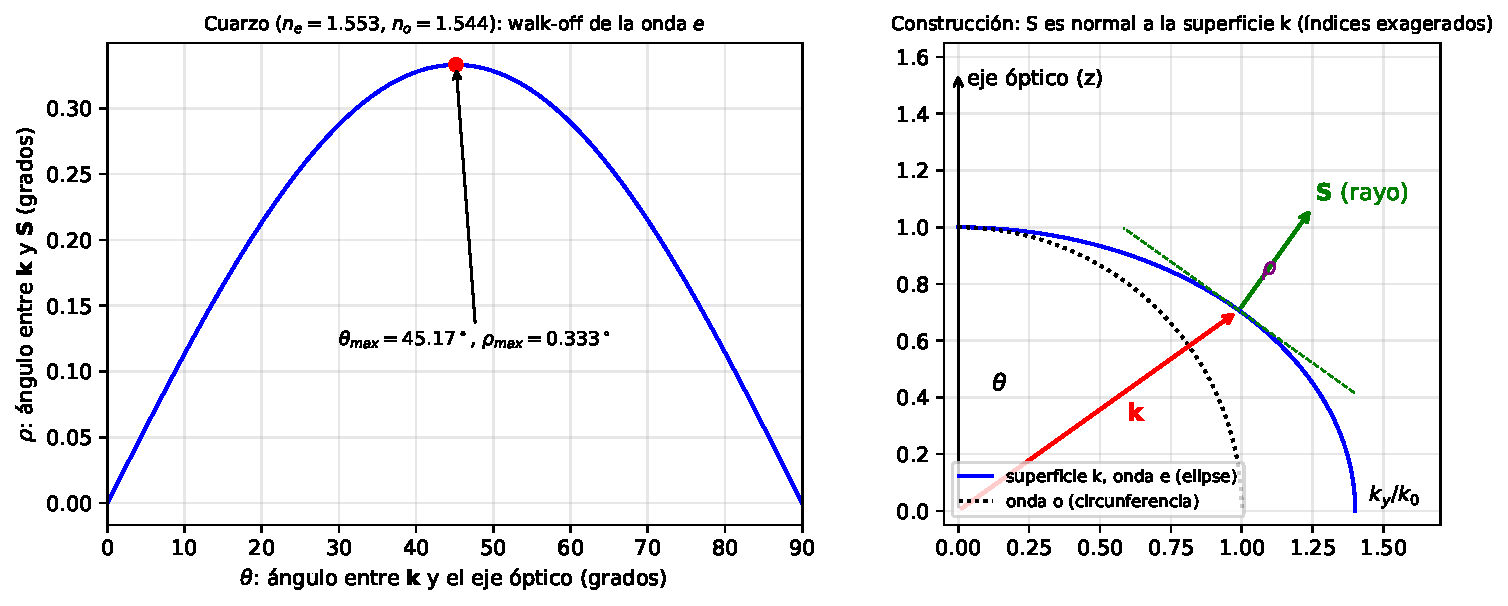
\includegraphics[width=\textwidth]{punto7_walkoff_cuarzo}
\caption{Izquierda: ángulo de walk-off \eqref{eq:walkoff} del cuarzo en función del ángulo
$\theta$ entre $\kv$ y el eje óptico, con el máximo en $\theta=45.17^\circ$. Derecha:
construcción con la superficie $k$ de la onda extraordinaria (elipse) y de la ordinaria
(circunferencia): el rayo $\Sv$ es normal a la elipse; los índices se han exagerado
($n_e/n_o=1.4$) para que la inclinación sea visible.}
\label{fig:p7}
\end{figure}

%=====================================================================
\section{Punto 8: Problema 6.6-2, rotación de polarización con una secuencia de polarizadores}
%=====================================================================

\emph{Una onda linealmente polarizada en $x$ atraviesa $N$ polarizadores lineales cuyos ejes de
transmisión están inclinados ángulos $m\theta$ ($m=1,2,\dots,N$; $\theta=\pi/2N$) respecto al
eje $x$. Demuestre que la luz transmitida está linealmente polarizada en $y$ pero su amplitud se
reduce en el factor $\cos^N\theta$. ¿Qué ocurre en el límite $N\to\infty$? Sugerencia: use
matrices de Jones y note que $\Rm[(m+1)\theta]\,\Rm(-m\theta)=\Rm(\theta)$.} (p.~242.)

\subsection*{Matriz de cada polarizador}

Un polarizador con eje de transmisión en $x$ tiene matriz $\Pm_x=\mathrm{diag}(1,0)$ (6.1-18).
Con el eje a un ángulo $m\theta$, por (6.1-24),
\[
\Pm_m=\Rm(-m\theta)\,\Pm_x\,\Rm(m\theta),
\qquad
\Rm(\theta)=\begin{bmatrix}\cos\theta&\sin\theta\\-\sin\theta&\cos\theta\end{bmatrix},
\]
que desarrollada es la (6.1-25),
$\Pm_m=\begin{bmatrix}\cos^2m\theta&\sin m\theta\cos m\theta\\ \sin m\theta\cos m\theta&\sin^2m\theta\end{bmatrix}$.

\subsection*{Producto de la cadena}

La luz pasa por $\Pm_1,\Pm_2,\dots,\Pm_N$ en ese orden, así que
\[
\Tm=\Pm_N\Pm_{N-1}\cdots\Pm_2\Pm_1
=\Rm(-N\theta)\Pm_x\underbrace{\Rm(N\theta)\Rm(-(N-1)\theta)}_{\Rm(\theta)}\Pm_x
\underbrace{\Rm((N-1)\theta)\Rm(-(N-2)\theta)}_{\Rm(\theta)}\Pm_x\cdots\Pm_x\,\Rm(\theta).
\]
Cada par de rotaciones consecutivas se contrae con la identidad de la sugerencia,
$\Rm[(m+1)\theta]\Rm(-m\theta)=\Rm(\theta)$ (las rotaciones de coordenadas se componen sumando
ángulos, $\Rm(\alpha)\Rm(\beta)=\Rm(\alpha+\beta)$), y queda
\[
\Tm=\Rm(-N\theta)\left[\Pm_x\Rm(\theta)\right]^N .
\]
El bloque elemental es
\[
\Pm_x\Rm(\theta)=\begin{bmatrix}1&0\\0&0\end{bmatrix}
\begin{bmatrix}\cos\theta&\sin\theta\\-\sin\theta&\cos\theta\end{bmatrix}
=\begin{bmatrix}\cos\theta&\sin\theta\\0&0\end{bmatrix}\equiv\mathbf{M},
\]
y sus potencias se calculan de inmediato porque $\mathbf M$ tiene rango 1:
\[
\mathbf M^2=\begin{bmatrix}\cos\theta&\sin\theta\\0&0\end{bmatrix}
\begin{bmatrix}\cos\theta&\sin\theta\\0&0\end{bmatrix}
=\begin{bmatrix}\cos^2\theta&\cos\theta\sin\theta\\0&0\end{bmatrix}=\cos\theta\,\mathbf M
\;\Longrightarrow\;
\mathbf M^N=\cos^{N-1}\theta\,\mathbf M .
\]
Por tanto
\[
\Tm=\cos^{N-1}\theta\;\Rm(-N\theta)\begin{bmatrix}\cos\theta&\sin\theta\\0&0\end{bmatrix}.
\]

\subsection*{Salida para la entrada polarizada en $x$}

Con $\Jv_1=[1,\,0]^T$:
\[
\mathbf M^N\Jv_1=\cos^{N-1}\theta\begin{bmatrix}\cos\theta\\0\end{bmatrix}=\cos^N\theta\begin{bmatrix}1\\0\end{bmatrix},
\qquad
\Jv_2=\Tm\Jv_1=\cos^N\theta\;\Rm(-N\theta)\begin{bmatrix}1\\0\end{bmatrix}
=\cos^N\theta\begin{bmatrix}\cos N\theta\\ \sin N\theta\end{bmatrix}.
\]
Con $N\theta=\pi/2$,
\[
\boxed{\;\Jv_2=\cos^N\!\left(\frac{\pi}{2N}\right)\begin{bmatrix}0\\1\end{bmatrix}\;}
\]
luz linealmente polarizada en $y$ (el eje del último polarizador) con la amplitud reducida en
$\cos^N\theta$ y la intensidad en $\cos^{2N}\theta$. El resultado tiene una lectura directa: cada
polarizador proyecta la polarización lineal que le llega sobre su eje, que forma $\theta$ con el
anterior, y la proyección multiplica la amplitud por $\cos\theta$; tras $N$ etapas, $\cos^N\theta$.
La polarización gira $\theta$ en cada etapa y termina en $N\theta=90^\circ$.

\subsection*{Límite $N\to\infty$}

Con $\theta=\pi/2N\to0$ se expande $\cos\theta=1-\theta^2/2+O(\theta^4)$ y
$\ln\cos\theta=-\theta^2/2+O(\theta^4)$:
\[
\cos^N\!\left(\frac{\pi}{2N}\right)=\exp\!\left[N\ln\cos\frac{\pi}{2N}\right]
=\exp\!\left[-\frac{\pi^2}{8N}+O\!\left(N^{-3}\right)\right]\xrightarrow[N\to\infty]{}1 .
\]
La amplitud transmitida tiende a 1 (la transmitancia $\cos^{2N}\theta\approx e^{-\pi^2/4N}\to1$):
una sucesión infinita de polarizadores con orientación que varía de forma continua gira la
polarización $90^\circ$ \emph{sin pérdida}, aunque la polarización de entrada y el último polarizador estén
cruzados. La polarización sigue al eje por proyecciones sucesivas: si el eje cambia poco entre
proyecciones consecutivas, la pérdida por etapa es de segundo orden en $\theta$ ($\sin^2\theta$) y la suma de
$N$ pérdidas de orden $1/N^2$ se anula como $1/N$. Es un análogo disipativo del cristal
líquido nemático torcido (§6.5): allí el medio es una cadena de retardadores sin pérdidas cuyo eje
gira lentamente ($\beta\gg\alpha$) y la polarización sigue al eje molecular; aquí se descarta
energía en cada proyección y la pérdida solo se anula para $N\to\infty$.

\begin{center}
\begin{tabular}{S[table-format=4] S[table-format=1.3] S[table-format=1.3]}
\toprule
{$N$} & {$\cos^N(\pi/2N)$} & {$\mathcal T=\cos^{2N}(\pi/2N)$}\\
\midrule
1 & 0 & 0\\
2 & 0.500 & 0.250\\
3 & 0.650 & 0.422\\
10 & 0.883 & 0.781\\
100 & 0.988 & 0.976\\
1000 & 0.999 & 0.998\\
\bottomrule
\end{tabular}
\end{center}

\begin{figure}[H]
\centering
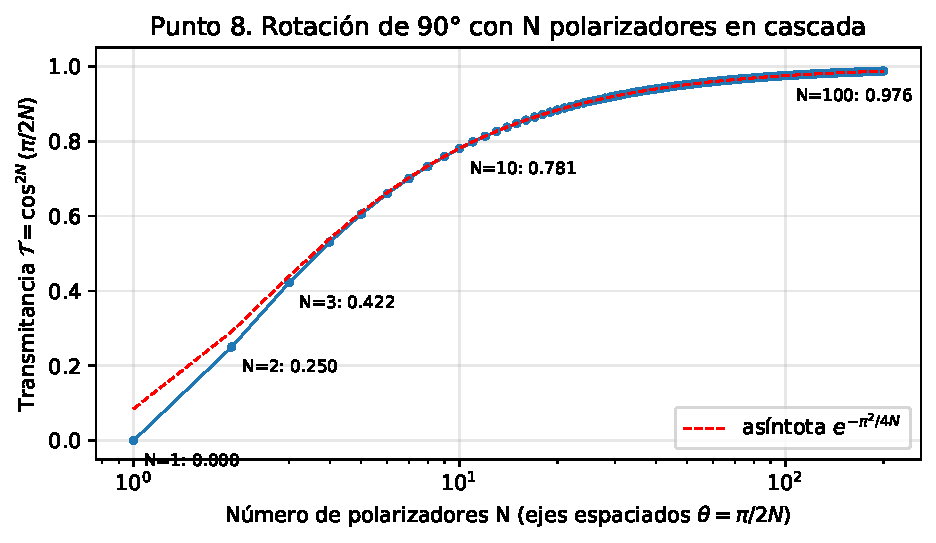
\includegraphics[width=0.7\textwidth]{punto8_transmitancia}
\caption{Transmitancia de potencia de la cadena de $N$ polarizadores que gira la polarización
$90^\circ$, y su asíntota $e^{-\pi^2/4N}$.}
\label{fig:p8}
\end{figure}

%=====================================================================
\appendix
\section{Código MATLAB del punto 4}
\label{ap:codigo}
%=====================================================================

Archivo \texttt{punto4\_pulso\_dispersion.m}. Está escrito para generar las figuras \ref{fig:p3},
\ref{fig:p4} y \ref{fig:p4b} y la Tabla~\ref{tab:p4}.

\lstinputlisting{punto4_pulso_dispersion.m}

\end{document}
